\documentclass[12pt,a4paper,oneside]{book}

\usepackage{subcaption}
\usepackage{listings}
\usepackage{tikz}
\usetikzlibrary{shapes.geometric, arrows.meta, positioning, fit, backgrounds, calc}

\lstset{
    basicstyle=\ttfamily\small,
    frame=single,
    breaklines=true,
    showstringspaces=false,
    numbers=none
}

% ---------- Idioma y codificación ----------
\usepackage[T1]{fontenc}
\usepackage[utf8]{inputenc}
\usepackage{float}
\usepackage{rotating}
\usepackage[spanish,es-tabla,es-nodecimaldot]{babel}

% ---------- Tipografía ----------
\usepackage{amsmath,amsthm}
\usepackage{mathpazo}     

% ---------- Página ----------
\usepackage[
  a4paper,
  top=3cm, bottom=2.5cm,
  inner=3.2cm, outer=2.5cm,
  headsep=1cm
]{geometry}
\usepackage{setspace}
\onehalfspacing              % Interlineado 1.5 
\usepackage{emptypage}       % Páginas en blanco sin encabezado

% ---------- Color de acento ----------
\usepackage{xcolor}
\definecolor{acento}{HTML}{000000}
\definecolor{gris}{HTML}{5A5A5A}

% ---------- Gráficos, tablas y figuras ----------
\usepackage{graphicx}
\graphicspath{{figuras/}}
\usepackage{array}
\newcolumntype{L}[1]{>{\raggedright\arraybackslash}p{#1}}
\usepackage{booktabs}
\usepackage{tabularx}
\usepackage[font=small,labelfont={bf,color=acento}]{caption}

% ---------- Matemáticas ----------
\usepackage{amssymb}

% ---------- Listas y varios ----------
\usepackage{enumitem}
\setlist{itemsep=2pt,topsep=4pt}

% ---------- Código fuente ----------

% ---------- Títulos de capítulo y sección ----------
\usepackage{titlesec}
\titleformat{\chapter}[display]
  {\normalfont\sffamily\huge\bfseries\color{acento}}
  {\filleft\fontsize{64}{64}\selectfont\color{acento!25}\thechapter}
  {-6pt}
  {\filleft\Huge}
  [\vspace{4pt}{\color{acento}\titlerule[1.2pt]}]
\titleformat{name=\chapter,numberless}[display]
  {\normalfont\sffamily\huge\bfseries\color{acento}}
  {}
  {0pt}
  {\filleft\Huge}
  [\vspace{4pt}{\color{acento}\titlerule[1.2pt]}]
\titlespacing*{\chapter}{0pt}{-30pt}{30pt}

\titleformat{\section}{\normalfont\sffamily\Large\bfseries\color{acento}}{\thesection}{1em}{}
\titleformat{\subsection}{\normalfont\sffamily\large\bfseries\color{acento!85}}{\thesubsection}{1em}{}

% ---------- Encabezados y pies ----------
\usepackage{fancyhdr}
\pagestyle{fancy}
\fancyhf{}
\renewcommand{\headrulewidth}{0.4pt}
\fancyhead[L]{\small\nouppercase{\leftmark}}
\fancyhead[R]{\small\thepage}
\fancypagestyle{plain}{\fancyhf{}\renewcommand{\headrulewidth}{0pt}\fancyfoot[C]{\small\thepage}}

% ---------- Teoremas ----------
\theoremstyle{plain}
\newtheorem{teorema}{Teorema}[chapter]
\newtheorem{lema}[teorema]{Lema}
\newtheorem{proposicion}[teorema]{Proposición}
\newtheorem{corolario}[teorema]{Corolario}
\theoremstyle{definition}
\newtheorem{definicion}[teorema]{Definición}
\newtheorem{ejemplo}[teorema]{Ejemplo}
\theoremstyle{remark}
\newtheorem{observacion}[teorema]{Observación}

% ---------- Bibliografía ----------
\usepackage{csquotes}
\usepackage[backend=biber,style=ieee,natbib=true]{biblatex}
\addbibresource{bibliografia.bib}
% ============================================================
%  DATOS 
% ============================================================
\newcommand{\eltitulo}{Prototipo de sistema de detección de caídas en adultos mayores mediante visión artificial.}
\newcommand{\elsubtitulo}{Trabajo Terminal No. A083}
\newcommand{\elautoruno}{Pardo Cordova Alonso}
\newcommand{\elautordos}{Sanchez Flores María Fernanda}
\newcommand{\eldirectoruno}{Correa Coyac David}
\newcommand{\eldirectordos}{Dr. Vázquez Gómez Juan Irving}
\newcommand{\launiversidad}{Instituto Politécnico Nacional}
\newcommand{\lafacultad}{Escuela Superior de Cómputo}
\newcommand{\lacarrerauno}{Ingeniería en Sistemas Computacionales}
\newcommand{\lacarrerados}{Ingeniería en Inteligencia Artificial}
\newcommand{\lafecha}{Noviembre de 2026}

% ---------- Enlaces ----------
\usepackage[hyperfootnotes=false]{hyperref}
\hypersetup{
  colorlinks=true,
  linkcolor=acento,
  citecolor=acento,
  urlcolor=acento,
  pdftitle={\eltitulo},
  pdfauthor={\elautoruno, \elautordos}
}
\urlstyle{same}   % URLs con la misma letra del texto

% ============================================================
\begin{document}

% ------------------------------------------------------------
%  PORTADA
% ------------------------------------------------------------
\begin{titlepage}
\thispagestyle{empty}
\centering


\includegraphics[height=2.2cm]{Figuras/ipn.png}

\includegraphics[height=2.2cm]{Figuras/escom.png}\\[1.5 cm]

{\sffamily\bfseries\large\scshape \launiversidad \par}
\vspace{0.25cm}
{\sffamily\large\scshape \lafacultad \par}
\vspace{0.5cm}

{\color{acento}\rule{0.6\linewidth}{0.8pt}}\par
\vfill

% Bloque de Título
{\sffamily\LARGE\bfseries\color{acento} \eltitulo \par}
\vspace{0.4cm}
{\large\itshape \elsubtitulo \par}

\vfill

% Grados / Carreras
{\small\scshape Presentado por las carreras de:\par}
\vspace{0.25cm}
{\normalsize\bfseries \lacarrerauno \par}
{\normalsize\bfseries \lacarrerados \par}

\vfill

% Autores y Directores 
\noindent
\begin{minipage}[t]{0.48\textwidth}
  \centering
  {\footnotesize\bfseries\scshape Presentan\par}
  \vspace{0.25cm}
  {\normalsize \elautoruno \par}
  \vspace{0.15cm}
  {\normalsize \elautordos \par}
\end{minipage}
\hfill
\begin{minipage}[t]{0.48\textwidth}
  \centering
  {\footnotesize\bfseries\scshape Dirección\par}
  \vspace{0.25cm}
  {\normalsize \eldirectoruno \par}
  \vspace{0.15cm}
  {\normalsize \eldirectordos \par}
\end{minipage}

\vfill
{\footnotesize \lafecha \par}

\end{titlepage}

% ------------------------------------------------------------
%  PÁGINAS PRELIMINARES
% ------------------------------------------------------------
\frontmatter
\pagestyle{plain}


% --- Resumen ---
\chapter*{Resumen}
\addcontentsline{toc}{chapter}{Resumen}
\markboth{Resumen}{Resumen}

Las caídas son una de las principales causas de lesiones y muerte en las personas adultas mayores, y sus consecuencias se agravan cuando la ayuda tarda en llegar, como ocurre en los hogares unipersonales. Las soluciones actuales dependen de dispositivos que el usuario debe portar o activar o, en el caso de los sistemas de visión artificial, enfrentan problemas de privacidad, falsas alarmas y alto costo de cómputo. Este Trabajo Terminal propone un prototipo de sistema de detección de caídas basado en visión artificial que, mediante una cámara RGB y una placa Edge basada en Raspberry Pi 5, estima el esqueleto de la persona con el modelo YOLO26-pose, clasifica su postura en cada cuadro y analiza la secuencia de posturas para identificar una caída. El video se procesa localmente y no se almacena; ante una caída, el sistema publica una alerta mediante el protocolo MQTT y una aplicación móvil Android notifica a un tutor, quien confirma o descarta el evento. El desarrollo sigue la metodología CRISP-ML(Q), que integra en un solo ciclo de vida el modelo de aprendizaje automático y la infraestructura IoT. En esta primera etapa se presentan el estado del arte, el marco teórico, los requisitos del sistema y del modelo, los criterios de éxito, entre ellos una sensibilidad y una especificidad de al menos 90\,\%, y el diseño de la arquitectura IoT, del flujo de adquisición de video, de la estrategia de preprocesamiento de datos y de las interfaces de la aplicación móvil. Estos resultados constituyen la base para la implementación, el entrenamiento y la evaluación del prototipo en la segunda etapa del proyecto.


\vspace{1em}
\noindent\textbf{Palabras clave:} Aprendizaje profundo, Detección de caídas en adultos mayores, Cómputo en el borde, Internet de las cosas, Visión artificial basada en esqueletos.

% --- Abstract ---
\chapter*{Abstract}
\addcontentsline{toc}{chapter}{Abstract}
\markboth{Abstract}{Abstract}
 
\begin{otherlanguage}{english}
Falls are one of the leading causes of injury and death among older adults, and their consequences worsen when help is delayed, as often happens in single-person households. Current solutions rely on devices that the user must wear or activate, while vision-based systems face privacy concerns, false alarms, and high computational cost. This project proposes a prototype fall detection system based on computer vision that, using an RGB camera and a Raspberry Pi 5 edge device, estimates the person's skeleton with the YOLO26-pose model, classifies their posture in each frame, and analyzes the sequence of postures to identify a fall. Video is processed locally and never stored; when a fall is detected, the system publishes an alert through the MQTT protocol, and an Android mobile application notifies a caregiver, who confirms or dismisses the event. Development follows the CRISP-ML(Q) methodology, which integrates the machine learning model and the IoT infrastructure into a single life cycle. This first stage presents the state of the art, the theoretical framework, the system and model requirements, the success criteria, including a sensitivity and specificity of at least 90\%, and the design of the IoT architecture, the video acquisition flow, the data preprocessing strategy, and the mobile application interfaces. These results lay the foundation for the implementation, training, and evaluation of the prototype in the second stage of the project.


\vspace{1em}
\noindent\textbf{Keywords:} Deep learning, Fall detection in older adults, Edge computing, Internet of things, Skeleton-based computer vision.
\end{otherlanguage}

% --- Índices ---
\cleardoublepage
\tableofcontents
\cleardoublepage
\listoffigures
\addcontentsline{toc}{chapter}{\listfigurename}
\cleardoublepage
\listoftables
\addcontentsline{toc}{chapter}{\listtablename}

% ------------------------------------------------------------
%  CUERPO DE LA TESIS
% ------------------------------------------------------------
\mainmatter
\pagestyle{fancy}

% ============================================================
\chapter{Generalidades}
\label{cap:generalidades}

\section{Introducción}
En la actualidad, la población de adultos mayores es partícipe de un cambio demográfico significativo; se estima que para el año 2050 la población de 65 años alcanzará los 1,500 millones \parencite{nahian2026ai}. Por lo que preservar su bienestar y calidad de vida ha sido un tema que ha cobrado mayor importancia. En México, se han creado diversos programas, créditos y apoyos con este propósito \parencite{inapam2015alerta}; sin embargo, no cubren uno de los principales peligros que corre este sector de la población, los accidentes.

El sector de la población de adultos mayores es altamente vulnerable a caídas accidentales: a nivel mundial, entre el 28\% y el 35\% de las personas mayores de 65 años sufren al menos una caída al año \parencite{who2008falls}, y las caídas representan la segunda causa mundial de muerte por traumatismos involuntarios \parencite{who2021caidas}.

La falta de vigilancia, o pertenecer a un hogar unipersonal, pueden ser factores que afecten a la pronta atención en este tipo de accidentes, lo que, para esta población, puede tener consecuencias graves, como fracturas, traumatismos craneoencefálicos, contusiones, traumas cerebrales, pérdida de la autonomía o, en el peor de los casos, fallecimiento \parencite{cenidsp2023caidas}.

Existen diversos enfoques que han intentado proponer soluciones para este problema, o similares, a través de Sistemas de Detección de Caídas (FDS) categorizados en sensores vestibles (wearables), ambientales y de visión artificial \parencite{nahian2026ai}. Aunque los sistemas de visión ofrecen una alta precisión al capturar características espaciotemporales ricas, enfrentan dos retos críticos: la invasión a la privacidad del usuario en áreas sensibles, como dormitorios o baños, y la alta tasa de falsos positivos generados por actividades de la vida diaria (ADL) \parencite{nahian2026ai}. Esta confusión suele darse porque acciones cotidianas, como recostarse rápidamente, agacharse de golpe a recoger un objeto o sentarse, comparten trayectorias de movimiento y cambios bruscos de velocidad muy similares a los de una caída real.

Ante esta problemática, el presente Trabajo Terminal se plantea como una solución tecnológica de primera línea de defensa mediante un sistema basado en visión artificial que utiliza cámara RGB para la extracción de esqueletos humanos. Este enfoque permite analizar la dinámica del movimiento sin procesar ni almacenar video completo, ya que el procesamiento local reduce la exposición de datos y favorece la privacidad. Además, para minimizar el impacto de las falsas alarmas, se integra una capa de validación humana mediante una notificación móvil a un tutor, permitiendo una toma de decisiones informada antes de activar servicios de emergencia.

\section{Planteamiento del problema}
Las caídas son uno de los principales riesgos para la salud de las personas adultas mayores. Se estima que entre el 28\,\% y el 35\,\% de las personas de 65 años o más sufren al menos una caída al año, proporción que aumenta a entre el 32\,\% y el 42\,\% en las mayores de 70 años \parencite{who2008falls}. Además de las lesiones físicas, una caída puede desencadenar un síndrome poscaída que incluye dependencia, pérdida de autonomía, inmovilización y depresión, así como el temor a no poder levantarse después de caer \parencite{who2008falls}.
 
La gravedad de estas consecuencias depende en buena medida del tiempo que transcurre entre la caída y la llegada de ayuda. Este tiempo crece cuando la persona vive sola o pasa periodos prolongados sin supervisión, situación que además se asocia con un mayor riesgo de caer \parencite{who2008falls}. En un hogar unipersonal, si el adulto mayor queda inconsciente, lesionado o simplemente no puede incorporarse, puede permanecer en el suelo hasta que alguien note su ausencia.
 
Las soluciones disponibles no resuelven este problema por completo. Los botones de pánico y los dispositivos portables con acelerómetro dependen de que el usuario los lleve puestos, los mantenga cargados y, en el caso de los botones, de que esté consciente para activarlos \parencite{igual2013challenges}. Los sistemas basados en visión artificial no requieren la colaboración del usuario, pero enfrentan tres retos: la privacidad, porque implican colocar cámaras dentro de la vivienda; las falsas alarmas, porque actividades cotidianas como sentarse o acostarse con rapidez producen movimientos parecidos a una caída; y el costo de cómputo, porque los modelos de aprendizaje profundo suelen requerir hardware potente o servidores en la nube \parencite{alam2022review}. Asimismo, la mayoría de los trabajos reportados se evalúan fuera de línea con caídas simuladas y no llegan a integrarse en un sistema que notifique a un cuidador \parencite{igual2013challenges,alam2022review}.
 
Por lo anterior, se identifica la necesidad de un sistema que detecte caídas de forma automática, sin depender de que el adulto mayor porte o active algún dispositivo; que procese el video localmente para no exponer imágenes de la vivienda; que distinga una caída de las actividades de la vida diaria con una tasa baja de falsas alarmas; y que notifique de inmediato a un tutor para que pueda verificar la situación y actuar.
 
De ahí surge la pregunta que guía este trabajo: \textit{¿es posible detectar caídas de adultos mayores en tiempo real, a partir del análisis de la secuencia de posturas del esqueleto obtenido de una cámara RGB y procesado en un dispositivo de borde, con la sensibilidad y especificidad necesarias para alertar oportunamente a un tutor?}

\section{Justificación}
El presente Trabajo Terminal propone una solución técnica óptima para la detección de caídas, integrando metodologías que han demostrado resultados favorables en investigaciones anteriores. El enfoque primordial es salvaguardar la integridad física del adulto mayor mediante un monitoreo constante que permita reducir los tiempos de respuesta ante emergencias médicas.

A diferencia de sistemas convencionales, este proyecto busca optimizar la detección al implementar YOLO26, una arquitectura reciente de visión por computadora diseñada para el procesamiento en tiempo real. Esta se complementa con una placa Edge basada en Raspberry Pi 5, cuya selección se justifica en la Sección~\ref{sec:seleccion-placa}. El procesamiento local reduce la exposición de datos de los usuarios al evitar el almacenamiento de frames en la nube, promoviendo así su privacidad y seguridad.

La solución está orientada directamente a resolver la problemática de los hogares unipersonales, un sector donde investigaciones previas han confirmado la factibilidad técnica de la detección de caídas, pero donde aún existe una brecha en la implementación de sistemas no invasivos y de alta precisión que se adapten a la vida cotidiana del usuario.

La complejidad de esta solución exige integrar, en un solo sistema, las competencias de dos perfiles de ingeniería de la ESCOM, lo que justifica su desarrollo conjunto. Por un lado, la Ingeniería en Sistemas Computacionales orquesta la infraestructura de telecomunicaciones e Internet of Things (IoT), gestionando protocolos de baja latencia (MQTT) y construyendo la aplicación móvil nativa que cierra el ciclo de alerta. Por otro lado, la Ingeniería en Inteligencia Artificial aporta el rigor analítico requerido para el preprocesamiento de imágenes, balanceo de clases, ajuste de YOLO26 para la estimación de pose y entrenamiento del clasificador de posturas, optimizándolos para ejecutarse eficientemente en hardware de recursos limitados. Esta integración demuestra la calidad y aplicación de los conocimientos adquiridos en ambas carreras para un proyecto de titulación.

Finalmente, la implementación de este Trabajo Terminal prescinde de costosos servidores en la nube al apostar por una arquitectura basada en Edge Computing con placas de desarrollo más accesibles, asimismo, el uso de bibliotecas de código abierto para el modelo YOLO26 y el protocolo MQTT, en conjunto con el uso de datos públicos para el entrenamiento, permite que el proyecto se mantenga dentro de un presupuesto de bajo costo y pueda ejecutarse y evaluarse en el periodo académico establecido.


\section{Objetivos}
\subsection{Objetivo general}
Desarrollar un prototipo de sistema inteligente para la detección de caídas en adultos mayores, utilizando visión artificial basada en el análisis de esqueletos mediante cámara RGB y una plataforma de notificación móvil para contactos
de emergencia.

\subsection{Objetivos específicos}
\begin{enumerate}
    \item Configurar la arquitectura de adquisición de datos mediante el uso de cámaras RGB para obtener información del entorno.

    \item Implementar el modelo YOLO26 \parencite{ultralytics2026yolo26} para la estimación de pose y extracción de los puntos clave del esqueleto humano a través de imágenes RGB, obteniendo como salida las coordenadas (x, y) de un conjunto de keypoints (por ejemplo, nariz, ojos, hombros, codos, muñecas, caderas, rodillas, tobillos), optimizando el procesamiento para dispositivos edge; este procesamiento local reduce la exposición de datos y protege el anonimato del usuario.
 
    \item Entrenar un modelo de inteligencia artificial capaz de clasificar con precisión entre una caída real y actividades cotidianas (sentarse, caminar, acostarse) basándose en la secuencia de posturas del esqueleto.
 
    \item Desarrollar una aplicación móvil Android que reciba alertas ante una caída, permitiendo al contacto de emergencia visualizar el estado del evento.

    \item Evaluar el rendimiento del sistema utilizando las métricas de precisión, sensibilidad, especificidad y exactitud, validando el prototipo con conjuntos de datos públicos; de esta forma, el desempeño del sistema será evaluado para verificar su fiabilidad al discriminar verdaderas caídas frente a actividades de la vida diaria.
\end{enumerate}

\section{Alcances y limitaciones}
\label{sec:alcances}
 
\subsection{Alcances}
\begin{itemize}
  \item Se desarrollará un \textbf{prototipo funcional}, no un producto comercial, que integre la captura de video, la detección de caídas y la notificación al tutor.
  \item El sistema utilizará \textbf{una cámara RGB} conectada a una \textbf{placa Edge basada en Raspberry Pi 5}, donde se ejecutarán la estimación de pose con YOLO26 \citep{sapkota2025yolo26} el clasificador de posturas y el análisis temporal de la secuencia de posturas.
  \item El sistema está pensado para \textbf{una persona en una habitación interior} con iluminación artificial o natural suficiente.
  \item El clasificador reconocerá en cada cuadro cuatro posturas: \textbf{de pie}, \textbf{sentado}, \textbf{acostado} y \textbf{caído}; a partir de su secuencia, el sistema decidirá si ocurrió una \textbf{caída} o una actividad cotidiana, considerando caminar, sentarse, acostarse y agacharse.
  \item El modelo se entrenará y validará con \textbf{conjuntos de datos públicos} de caídas y actividades de la vida diaria, complementados con un conjunto de validación capturado por el equipo en condiciones controladas.
  \item Ante una caída, la placa publicará una alerta mediante \textbf{MQTT} y una \textbf{aplicación Android} notificará al tutor, quien podrá confirmar o descartar el evento.
  \item El desempeño se evaluará con sensibilidad, especificidad, precisión y exactitud, además de la tasa de procesamiento en la placa y el tiempo de extremo a extremo, conforme a los criterios de éxito de la Sección~\ref{sec:criterios-exito}.
\end{itemize}
 
\subsection{Limitaciones}
\begin{itemize}
  \item \textbf{Una sola persona en escena.} No se contemplan escenas con varias personas ni la identificación de quién cayó.
  \item \textbf{Campo de visión de una cámara.} Las caídas fuera del encuadre o con oclusiones importantes (muebles que cubren a la persona) pueden no detectarse.
  \item \textbf{Iluminación.} Al usar una cámara RGB, el sistema no está diseñado para operar en oscuridad total.
  \item \textbf{Caídas simuladas.} Por razones éticas no se registrarán caídas reales de adultos mayores; el entrenamiento y la evaluación se basan en caídas simuladas por voluntarios, por lo que el desempeño en condiciones reales puede ser menor \citep{igual2013challenges}.
  \item \textbf{Sin validación clínica.} El prototipo no se probará con adultos mayores ni en entornos hospitalarios, y no sustituye a un dispositivo médico certificado.
  \item \textbf{Sin contacto automático con servicios de emergencia.} El sistema notifica únicamente al tutor; la decisión de solicitar ayuda médica queda en manos de este.
  \item \textbf{Conectividad.} El envío de la alerta requiere que la placa y el teléfono del tutor tengan conexión de red LAN.
  \item \textbf{Plataforma móvil.} La aplicación se desarrollará solo para Android.
  \item \textbf{Sin almacenamiento de video.} Para proteger la privacidad no se guardan imágenes, por lo que el sistema no ofrece evidencia visual del evento.
  \item \textbf{Detección, no prevención.} El sistema identifica caídas ocurridas; no predice ni previene caídas.
\end{itemize}

% ---------- Parte de María Fernanda ----------
\section{Estado del arte}
\label{sec:estado-arte}

Los sistemas de detección de caídas se agrupan comúnmente en tres familias según el tipo de sensor que emplean: dispositivos portables (acelerómetros y giroscopios que la persona lleva consigo), sensores ambientales instalados en la vivienda (presión, vibración, infrarrojo) y sistemas basados en visión, que analizan imágenes de una o varias cámaras \parencite{igual2013challenges}. Los dispositivos portables ofrecen buena sensibilidad, pero dependen de que el adulto mayor los use y los mantenga cargados; los sistemas de visión, en cambio, no requieren la colaboración del usuario y pueden aprovechar cámaras de bajo costo \parencite{alam2022review}.

Dentro de los sistemas de visión, la tendencia de la última década ha sido sustituir los descriptores diseñados a mano por modelos de aprendizaje profundo, en particular redes neuronales convolucionales (CNN), modelos híbridos y redes recurrentes de tipo LSTM \parencite{alam2022review}. Una línea de trabajo que ha ganado relevancia consiste en no clasificar directamente la imagen completa, sino estimar primero la pose de la persona —un conjunto de puntos clave o \textit{keypoints} del cuerpo— y analizar después cómo cambia ese esqueleto en el tiempo. Este enfoque reduce la información a unas cuantas coordenadas por cuadro, lo que disminuye el costo de cómputo y hace al clasificador menos sensible al fondo, la iluminación o la ropa.

A continuación se describen los trabajos más cercanos a la propuesta.

\paragraph{Kwolek y Kepski (2014).} Presentaron un sistema que corre sobre una plataforma embebida (PandaBoard ES, procesador ARM de doble núcleo) y combina mapas de profundidad de un sensor Kinect con un acelerómetro portable \parencite{kwolek2014human}. Con este trabajo publicaron el \textit{UR Fall Detection Dataset}, con 30 secuencias de caídas y 30 de actividades de la vida diaria. Usando únicamente profundidad, su clasificador SVM obtuvo 90\,\% de exactitud y 80\,\% de especificidad; al añadir el acelerómetro alcanzó 98.33\,\% de exactitud. El trabajo muestra que la detección en el borde es viable, pero también que, sin sensores portables, la especificidad es el punto débil.

\paragraph{Martínez-Villaseñor et al. (2019).} Investigadores de la Universidad Panamericana, en la Ciudad de México, publicaron el \textit{UP-Fall Detection Dataset}, un conjunto multimodal con 17 participantes, cinco tipos de caída y seis actividades cotidianas (caminar, estar de pie, sentarse, recoger un objeto, saltar y acostarse), registrados con sensores inerciales, infrarrojos, electroencefalografía y dos cámaras \parencite{martinez2019upfall}. Es un referente nacional y una fuente pública de video etiquetado que puede utilizarse para entrenar clasificadores por trayectoria.

\paragraph{Lin et al. (2021).} Propusieron un esquema en dos etapas: extraer el esqueleto con OpenPose y clasificar la secuencia de esqueletos con redes recurrentes LSTM y GRU \parencite{lin2021openpose}. El trabajo es un antecedente directo de la arquitectura que se plantea en este proyecto, aunque OpenPose es un modelo pesado para ejecutarse en tiempo real sobre hardware embebido.

\paragraph{Mobasheri et al. (2022).} Utilizaron MediaPipe para extraer \textit{keypoints} de video del conjunto UP-Fall y construyeron características cinemáticas a partir de solo tres puntos (nariz, hombro y cadera): ángulos respecto a la horizontal, su velocidad de cambio y la relación de alturas entre nariz y cadera \parencite{mobasheri2022fall}. Una red LSTM sobre ventanas de 18 cuadros alcanzó hasta 98.5\,\% de exactitud. Este resultado sugiere que unos pocos puntos del esqueleto contienen suficiente información para distinguir una caída, lo que favorece modelos ligeros.

\paragraph{Limitaciones comunes.} Las revisiones del área coinciden en tres problemas \parencite{igual2013challenges,alam2022review}: (1) la mayoría de los conjuntos de datos contienen caídas simuladas por personas jóvenes, por lo que el rendimiento reportado suele disminuir en condiciones reales; (2) los modelos de aprendizaje profundo requieren mucho cómputo, lo que dificulta llevarlos a dispositivos IoT; y (3) las falsas alarmas frente a actividades parecidas a una caída, como acostarse o sentarse bruscamente, siguen siendo frecuentes.

La Tabla~\ref{tab:estado-arte} resume los trabajos revisados y los compara con la propuesta.

\begin{table}[htbp]
\centering
\caption{Comparación de trabajos relacionados con la propuesta.}
\label{tab:estado-arte}
\small
\begin{tabular}{L{2.6cm}L{2.8cm}L{3.0cm}L{3.4cm}}
\toprule
\textbf{Trabajo} & \textbf{Sensores} & \textbf{Método} & \textbf{Ejecución / alerta} \\
\midrule
\textcite{kwolek2014human} & Profundidad (Kinect) + acelerómetro & Umbrales + SVM & Plataforma embebida; sin aplicación para cuidador \\
\addlinespace
\textcite{martinez2019upfall} & Inerciales, infrarrojo, EEG y dos cámaras & RF, SVM, MLP, kNN & Conjunto de datos; no es un sistema desplegado \\
\addlinespace
\textcite{lin2021openpose} & Cámara RGB & OpenPose + LSTM/GRU & Servidor; sin despliegue en el borde \\
\addlinespace
\textcite{mobasheri2022fall} & Cámara RGB (video de UP-Fall) & MediaPipe + LSTM & Evaluación fuera de línea \\
\addlinespace
\textbf{Propuesta} & \textbf{Una cámara RGB} & \textbf{YOLO26-pose + clasificador de posturas con análisis temporal} & \textbf{Placa Edge (Raspberry Pi 5); alerta al tutor vía MQTT y aplicación Android} \\
\bottomrule
\end{tabular}
\end{table}
 
A diferencia de los trabajos anteriores, la propuesta integra en un solo prototipo la estimación de pose con un modelo diseñado para dispositivos de borde, YOLO26 \parencite{sapkota2025yolo26}, la clasificación de posturas con el análisis de su secuencia en el tiempo y la entrega de la alerta a un tutor mediante una aplicación móvil. Además, solo requiere una cámara RGB convencional y no depende de que el adulto mayor porte algún dispositivo.

% ------------------------------------------------------------

\section{Metodología}
\label{sec:metodologia}

Para el desarrollo del prototipo se adopta CRISP-ML(Q) (\textit{Cross-Industry Standard Process for the development of Machine Learning applications with Quality assurance methodology}), un modelo de proceso propuesto por \textcite{studer2021crispmlq} que extiende CRISP-DM con las tareas propias del aprendizaje automático y añade, en cada fase, actividades de aseguramiento de la calidad orientadas a identificar y mitigar riesgos.

Se eligió CRISP-ML(Q) porque el componente central del sistema es un modelo de aprendizaje automático y todo lo demás —la captura de video, la placa Edge, la comunicación MQTT y la aplicación móvil— existe para alimentar a ese modelo y llevar su resultado al tutor. Por ello el proyecto se gestiona como \textbf{un solo sistema} que recorre un mismo ciclo de vida, y no como dos sistemas independientes que se integran al final: en cada fase se trabajan simultáneamente los aspectos del modelo y los de la infraestructura que lo soporta.

CRISP-ML(Q) consta de seis fases. La Tabla~\ref{tab:fases-crisp} muestra cómo se aplica cada una al proyecto.

\begin{table}[htbp]
\centering
\caption{Fases de CRISP-ML(Q) aplicadas al proyecto.}
\label{tab:fases-crisp}
\small
\begin{tabular}{L{3.0cm}L{6.0cm}L{3.2cm}}
\toprule
\textbf{Fase} & \textbf{Actividades en el proyecto} & \textbf{Periodo} \\
\midrule
1. Comprensión del negocio y de los datos & Requisitos del sistema y del modelo, criterios de éxito conjuntos (métricas, FPS, latencia de alerta), arquitectura IoT, flujos de alerta y mockups de la aplicación. & Ago -- oct 2026 (TT1) \\
\addlinespace
2. Preparación de los datos & Selección de conjuntos de datos públicos, estrategia de preprocesamiento de imágenes RGB y diseño del flujo de adquisición (resolución, FPS, formato de cuadros). Aumento de datos y balanceo de clases. & Sep -- oct 2026 (TT1); ene 2027 (TT2) \\
\addlinespace
3. Ingeniería del modelo & Estimación de pose y extracción de esqueletos; entrenamiento del clasificador de posturas y ajuste de la regla temporal; configuración de la Raspberry Pi 5 y medición de modelos candidatos en el hardware; conversión a formato ligero. & Oct -- nov 2026 (TT1); ene -- mar 2027 (TT2) \\
\addlinespace
4. Evaluación & Cálculo de sensibilidad, especificidad, precisión y exactitud; pruebas de integración de extremo a extremo (latencia, MQTT, entrega de alertas) contra los criterios de éxito de la fase 1. & Abr -- may 2027 \\
\addlinespace
5. Despliegue & Aplicación móvil, broker MQTT, notificaciones y scripts que convierten la inferencia en alerta al tutor. & Feb -- abr 2027 \\
\addlinespace
6. Monitoreo y mantenimiento & Registro de eventos y de la respuesta del tutor; análisis de falsos positivos a partir de las alertas descartadas. & May 2027 \\
\bottomrule
\end{tabular}
\end{table}

\paragraph{Aseguramiento de la calidad.} Siguiendo el enfoque de CRISP-ML(Q), al cierre de cada fase se verifica que sus entregables cumplan lo necesario para la siguiente y se registran los riesgos detectados. Los principales riesgos identificados desde la fase 1 son: (1) que el modelo no alcance las métricas objetivo con caídas reales, dado que los datos públicos contienen caídas simuladas; (2) que el modelo no alcance la tasa de cuadros requerida en la Raspberry Pi 5; y (3) que las falsas alarmas reduzcan la confianza del tutor en el sistema. Estos riesgos se atienden, respectivamente, con un conjunto de validación capturado en condiciones reales, con la medición temprana de modelos candidatos en el hardware y con el análisis de las alertas descartadas en la fase 6.

\paragraph{Iteración.} Como lo plantea el modelo, las fases no son estrictamente secuenciales: si en la evaluación no se alcanzan los criterios de éxito, se regresa a la preparación de los datos o a la ingeniería del modelo antes de continuar con el despliegue.

% ============================================================
\chapter{Marco teórico}
\label{cap:marco}

% ---------- Parte de María Fernanda (IA) ----------
\section{Visión artificial}
\label{sec:vision-artificial}

La visión artificial es el campo que busca que una computadora extraiga información útil de imágenes o video: reconocer objetos, ubicar personas o interpretar movimientos \parencite{szeliski2022computer}. Para una computadora, una imagen digital en color es una matriz de tamaño $H \times W \times 3$, donde $H$ y $W$ son el alto y el ancho en píxeles y cada píxel guarda tres intensidades, normalmente entre 0 y 255, para los canales rojo, verde y azul (RGB). Un video es una secuencia de estas imágenes, llamadas cuadros (\textit{frames}), capturadas a una tasa determinada que se expresa en cuadros por segundo (FPS).

En este proyecto la visión artificial se usa para dos tareas encadenadas: localizar a la persona en cada cuadro y estimar la posición de sus articulaciones, de modo que el análisis posterior se haga sobre el esqueleto y no sobre los píxeles.

\section{Aprendizaje profundo y redes convolucionales}
\label{sec:cnn}

El aprendizaje profundo es una rama del aprendizaje automático que utiliza redes neuronales de muchas capas para aprender representaciones de los datos directamente a partir de ejemplos, sin que una persona tenga que diseñar las características a mano \parencite{lecun2015deep,goodfellow2016deep}. Cada capa transforma su entrada en una representación un poco más abstracta; los parámetros de todas las capas se ajustan durante el entrenamiento minimizando una función de pérdida mediante descenso por gradiente y retropropagación.

Las redes neuronales convolucionales (CNN) son la arquitectura dominante para imágenes. En lugar de conectar cada neurona con todos los píxeles, una capa convolucional aplica pequeños filtros que recorren la imagen, de modo que los mismos pesos detectan un patrón (un borde, una textura, una parte del cuerpo) en cualquier posición. Al apilar capas convolucionales, de activación no lineal y de reducción de resolución, la red pasa de detectar bordes en las primeras capas a reconocer formas completas en las últimas \parencite{lecun2015deep}.

\section{Detección de objetos con YOLO}
\label{sec:yolo}

La detección de objetos consiste en localizar, mediante cajas delimitadoras, cada objeto de interés en una imagen y asignarle una clase. La familia de modelos YOLO (\textit{You Only Look Once}) resuelve esta tarea en una sola pasada de la red: divide la imagen en una cuadrícula y, para cada región, predice simultáneamente las cajas y las clases \parencite{redmon2016yolo}. Esta formulación de una sola etapa es la que permite a YOLO operar en tiempo real, por lo que se ha convertido en la opción habitual para aplicaciones con restricciones de latencia.

YOLO26, presentado por Ultralytics en septiembre de 2025, es una versión orientada explícitamente a dispositivos de borde \parencite{sapkota2025yolo26}. Sus cambios principales son: inferencia de extremo a extremo sin supresión de no máximos (NMS), lo que elimina un paso de posprocesamiento costoso; la eliminación de la pérdida \textit{Distribution Focal Loss}, que simplifica la exportación a otros formatos; y nuevas estrategias de entrenamiento (ProgLoss, STAL y el optimizador MuSGD). El modelo admite cinco tareas, entre ellas la estimación de pose, y puede exportarse a formatos ligeros como ONNX, TensorRT, TFLite y OpenVINO \parencite{sapkota2025yolo26}.

\section{Estimación de pose humana}
\label{sec:pose}

La estimación de pose humana consiste en localizar en una imagen un conjunto predefinido de puntos clave (\textit{keypoints}) del cuerpo, como hombros, codos, caderas, rodillas y tobillos. Al unir esos puntos se obtiene un esqueleto que describe la postura de la persona de forma compacta.

El esquema más usado es el del conjunto de datos COCO \parencite{lin2014coco}, que define 17 puntos clave: nariz, ojos, orejas, hombros, codos, muñecas, caderas, rodillas y tobillos (izquierdos y derechos). Para cada punto, el modelo entrega sus coordenadas $(x, y)$ en la imagen y un valor de confianza. Así, la postura de una persona en un cuadro queda representada por un vector de $17 \times 3 = 51$ valores, mucho más pequeño que la imagen original.

Existen dos enfoques generales. Los métodos \textit{bottom-up}, como OpenPose \parencite{cao2017openpose}, detectan primero todos los puntos clave de la imagen y después los agrupan por persona. Los métodos \textit{top-down} detectan primero a cada persona y luego estiman sus puntos dentro de la caja. YOLO-Pose \parencite{maji2022yolopose} propuso un tercer camino: extender el detector YOLO para que, en la misma pasada en que predice la caja de cada persona, prediga también sus 17 puntos clave. Los modelos de pose de YOLO26 siguen esta idea, lo que permite obtener el esqueleto con el costo de una sola inferencia.

\paragraph{Pose y detección de caídas.} Una caída se caracteriza por cambios rápidos en la geometría del cuerpo: el centro de masa desciende bruscamente, el tronco pasa de vertical a horizontal y la cabeza queda a una altura similar a la de la cadera. Estas señales pueden medirse directamente a partir de las coordenadas de los puntos clave a lo largo de varios cuadros, como lo muestran trabajos que alcanzan buenos resultados usando solo unos pocos puntos \parencite{mobasheri2022fall}.

\section{Análisis temporal de posturas}
\label{sec:secuencias}
 
Una sola postura no basta para distinguir una caída de una actividad normal: una persona acostada en la cama y una persona en el suelo tras caer pueden tener esqueletos parecidos. Lo que las diferencia es cómo se llegó a esa postura y cuánto tiempo se mantiene. Por ello, el análisis se realiza en dos niveles: primero se clasifica la postura de la persona en cada cuadro y después se analiza la secuencia de posturas de los últimos segundos.
 
Este enfoque descompone el problema en dos tareas más simples. El clasificador de posturas trabaja con un solo esqueleto a la vez, lo que permite entrenarlo con imágenes individuales y lo mantiene ligero para la placa Edge. El análisis temporal, por su parte, busca patrones característicos de una caída en la secuencia, como una transición rápida de una postura erguida a una postura en el suelo seguida de un periodo de inmovilidad.
 
Una alternativa es clasificar directamente secuencias de puntos clave con redes neuronales recurrentes. Las redes LSTM (\textit{Long Short-Term Memory}) añaden compuertas que controlan qué información se guarda, se olvida o se emite, lo que les permite aprender dependencias a lo largo de muchos pasos de tiempo \parencite{hochreiter1997lstm}, y se han usado con buenos resultados para detectar caídas a partir de esqueletos \parencite{lin2021openpose,mobasheri2022fall}. Sin embargo, requieren video etiquetado cuadro a cuadro y un mayor costo de cómputo, por lo que en este trabajo se adopta el análisis de la secuencia de posturas y se reserva el uso de modelos recurrentes como posible mejora.

\section{Métricas de evaluación}
\label{sec:metricas}

La decisión final del sistema es binaria: para cada secuencia de posturas analizada determina si ocurrió una caída (clase positiva) o no (clase negativa). Al comparar sus predicciones con las etiquetas reales se obtienen cuatro cantidades, que se organizan en la matriz de confusión (Tabla~\ref{tab:matriz-confusion}):

\begin{itemize}
  \item \textbf{Verdaderos positivos (VP):} caídas detectadas correctamente.
  \item \textbf{Falsos negativos (FN):} caídas que el sistema no detectó.
  \item \textbf{Falsos positivos (FP):} actividades normales que el sistema reportó como caída (falsas alarmas).
  \item \textbf{Verdaderos negativos (VN):} actividades normales clasificadas correctamente.
\end{itemize}

\begin{table}[htbp]
\centering
\caption{Matriz de confusión para la detección de caídas.}
\label{tab:matriz-confusion}
\begin{tabular}{lcc}
\toprule
 & \textbf{Predicción: caída} & \textbf{Predicción: no caída} \\
\midrule
\textbf{Real: caída} & VP & FN \\
\addlinespace
\textbf{Real: no caída} & FP & VN \\
\bottomrule
\end{tabular}
\end{table}

A partir de ellas se definen las cuatro métricas que se usan en este trabajo \parencite{sokolova2009systematic}:

\begin{align}
\text{Sensibilidad} &= \frac{VP}{VP + FN} \label{eq:sensibilidad}\\[4pt]
\text{Especificidad} &= \frac{VN}{VN + FP} \label{eq:especificidad}\\[4pt]
\text{Precisión} &= \frac{VP}{VP + FP} \label{eq:precision}\\[4pt]
\text{Exactitud} &= \frac{VP + VN}{VP + VN + FP + FN} \label{eq:exactitud}
\end{align}

La \textbf{sensibilidad} (o \textit{recall}) indica qué proporción de las caídas reales se detectó; es la métrica más importante para la seguridad del adulto mayor, porque cada falso negativo es una caída sin atender. La \textbf{especificidad} indica qué proporción de las actividades normales se reconoció como tal; una especificidad baja produce falsas alarmas que, con el tiempo, hacen que el tutor deje de confiar en el sistema. La \textbf{precisión} indica qué proporción de las alertas emitidas corresponde a caídas reales. Finalmente, la \textbf{exactitud} resume el desempeño global, pero puede ser engañosa cuando las clases están desbalanceadas, como ocurre en la práctica, donde las caídas son mucho menos frecuentes que las actividades cotidianas \parencite{sokolova2009systematic}. Por ello se reportan las cuatro métricas y no solo la exactitud.

\section{Cómputo en el borde}
\label{sec:edge}

El cómputo en el borde (\textit{edge computing}) consiste en procesar los datos en un dispositivo cercano al lugar donde se generan, en este caso una placa conectada a la cámara, en lugar de enviarlos a un servidor remoto. Para la detección de caídas esto tiene dos ventajas: reduce la latencia, porque la decisión se toma localmente, y protege la privacidad, porque el video no sale de la vivienda; solo se transmite la alerta. A cambio, la placa tiene memoria y capacidad de cómputo limitadas, lo que obliga a usar modelos compactos y formatos de ejecución optimizados, una de las dificultades señaladas por la literatura para llevar el aprendizaje profundo a dispositivos IoT \parencite{alam2022review}.

% ---------- Parte de Alonso (sistemas) ----------
\section{Internet de las cosas y protocolo MQTT}
El Internet de las Cosas (IoT, por sus siglas en inglés) interconecta objetos cotidianos con redes de datos, permitiendo el monitoreo y control de entornos físicos en tiempo real sin requerir interacción manual \parencite{ibm2026iot}. En el cuidado de adultos mayores, estas arquitecturas descentralizadas automatizan la recopilación de datos y la emisión de alertas tempranas hacia los responsables de la salud y familiares \parencite{ibm2026iot}. 

Para lograr una comunicación altamente reactiva entre la placa de procesamiento perimetral y el usuario final, se emplea MQTT (\textit{Message Queuing Telemetry Transport}). MQTT es un protocolo de mensajería ligero, diseñado para redes con recursos limitados o fluctuaciones de conexión, operando bajo un modelo ágil de publicación y suscripción (\textit{publish/subscribe}) \parencite{mqtt2026estandar}. Un servidor centralizado (\textit{broker}, como Mosquitto) gestiona la entrega de información organizada por jerarquías de tópicos, garantizando que el evento de caída detectado se transmita de forma confiable, con la urgencia y eficiencia que requieren los despliegues IoT domésticos \parencite{mqtt2026estandar}.

\section{Desarrollo de aplicaciones móviles Android}
Android es el sistema operativo móvil predominante basado en código abierto, cuyas capacidades nativas permiten un manejo robusto de procesos y eventos en segundo plano \parencite{uv2026desarrollo}. Al desarrollar la aplicación del tutor de forma nativa, el dispositivo móvil puede mantener un canal de suscripción persistente al \textit{broker} MQTT \parencite{mqtt2026estandar}. Esto asegura que en el instante exacto en que el sistema de visión clasifica un accidente, la aplicación despierte, intercepte el flujo de red y dispare inmediatamente las notificaciones de emergencia visuales y sonoras en la interfaz de usuario, optimizando radicalmente el tiempo de respuesta del cuidador \parencite{uv2026desarrollo}.

% ============================================================
\chapter{Análisis del sistema}
\label{cap:analisis}

% ---------- Parte de Alonso (sistemas) ----------
\section{Requisitos del sistema}
\label{sec:req-sistema}

En esta sección se definen las especificaciones que regulan el hardware, el software y los lineamientos de arquitectura IoT que habilitan la funcionalidad del prototipo. 

\subsection{Requisitos funcionales}
La Tabla~\ref{tab:rf-sis} especifica los requisitos funcionales que rigen la interacción entre el módulo de captura, el procesamiento local en la placa Edge, la publicación de alertas mediante el protocolo MQTT y la notificación en la aplicación móvil del tutor.
\begin{table}[htbp]
\centering
\caption{Requisitos funcionales del sistema IoT y de la aplicación móvil.}
\label{tab:rf-sis}
\small
\begin{tabular}{L{1.9cm}L{6.6cm}L{1.8cm}}
\toprule
\textbf{ID} & \textbf{Descripción} & \textbf{Prioridad} \\
\midrule
RF-001 & El subsistema de visión artificial deberá extraer las coordenadas $(x, y)$ de los puntos clave del esqueleto del usuario a partir de las imágenes RGB. & Alta \\
\addlinespace
RF-002 & El modelo de Inteligencia Artificial deberá analizar la secuencia de posturas del esqueleto para discriminar exitosamente entre una caída real y actividades de la vida diaria. & Alta \\
\addlinespace
RF-003 & La placa Edge deberá publicar una alerta crítica mediante el protocolo MQTT al obtener un resultado positivo de caída detectada. & Alta \\
\addlinespace
RF-004 & La placa Edge deberá omitir el procesamiento de notificaciones al clasificar negativamente el movimiento como una actividad cotidiana. & Alta \\
\addlinespace
RF-005 & La aplicación móvil del tutor deberá emitir una notificación de emergencia visual y sonora al recibir la señal MQTT del broker. & Alta \\
\bottomrule
\end{tabular}
\end{table}

\subsection{Requisitos no funcionales}
Con base en las características de calidad del producto definidas en el estándar internacional \textbf{ISO/IEC 25010}, se establecieron los requisitos no funcionales medibles del sistema en términos de seguridad y confidencialidad (privacidad local), adecuación funcional y fiabilidad (eficacia clasificatoria), eficiencia de desempeño (latencia de red en el \textit{broker} MQTT) y portabilidad/accesibilidad tecnológica (Tabla~\ref{tab:rnf-sis}).
\begin{table}[htbp]
\centering
\caption{Requisitos no funcionales de la arquitectura e infraestructura IoT.}
\label{tab:rnf-sis}
\small
\begin{tabular}{L{1.9cm}L{2.0cm}L{6.3cm}}
\toprule
\textbf{ID} & \textbf{Atributo} & \textbf{Descripción} \\
\midrule
RNF-001 & Privacidad & El subsistema de procesamiento local deberá retener el 100\,\% del flujo de imágenes en el dispositivo Edge para salvaguardar la privacidad en el hogar unipersonal. \\
\addlinespace
RNF-002 & Eficacia & El modelo de clasificación deberá alcanzar un rendimiento superior al 90\,\% en métricas de sensibilidad y especificidad para minimizar el impacto de falsas alarmas. \\
\addlinespace
RNF-003 & Latencia & El broker MQTT deberá entregar los mensajes de alerta con menos de 2 segundos de latencia de red para asegurar la pronta atención ante accidentes. \\
\addlinespace
RNF-004 & Accesibilidad & La arquitectura del sistema deberá operar con un 0\,\% de dependencia de servidores externos de pago, apoyándose completamente en tecnologías de código abierto. \\
\bottomrule
\end{tabular}
\end{table}

\subsection{Casos de uso del sistema IoT}
El flujo operativo principal obedece a un esquema transaccional de máquina a usuario, en el que el subsistema automatizado asume la responsabilidad analítica sin validaciones manuales previas. Los puntos críticos de interacción abarcan:

\begin{itemize}
    \item \textbf{Suministro ininterrumpido de video:} La cámara RGB (Capa de Percepción) alimenta la memoria RAM con el entorno óptico actual.
    \item \textbf{Extracción y clasificación en el Borde:} Como un evento incluido (\textit{include}), la placa procesadora extrae asíncronamente los nodos del esqueleto de cada cuadro y somete la sucesión de posturas a evaluación temporal.
    \item \textbf{Publicación autónoma de alertas:} Frente a un evento anómalo de caída (\textit{extend}), el microordenador actúa como cliente publicador para emitir un objeto JSON a un tópico dedicado (ej. \texttt{alertas/caidas}) a través del \textit{broker} Mosquitto.
    \item \textbf{Recepción y notificación móvil:} La aplicación Android del contacto de emergencia actúa como cliente permanente (\textit{suscriptor}), que recibe asíncronamente las alertas y desencadena un protocolo sonoro de emergencia en pantalla.
\end{itemize}
\begin{sidewaysfigure}
    \centering
    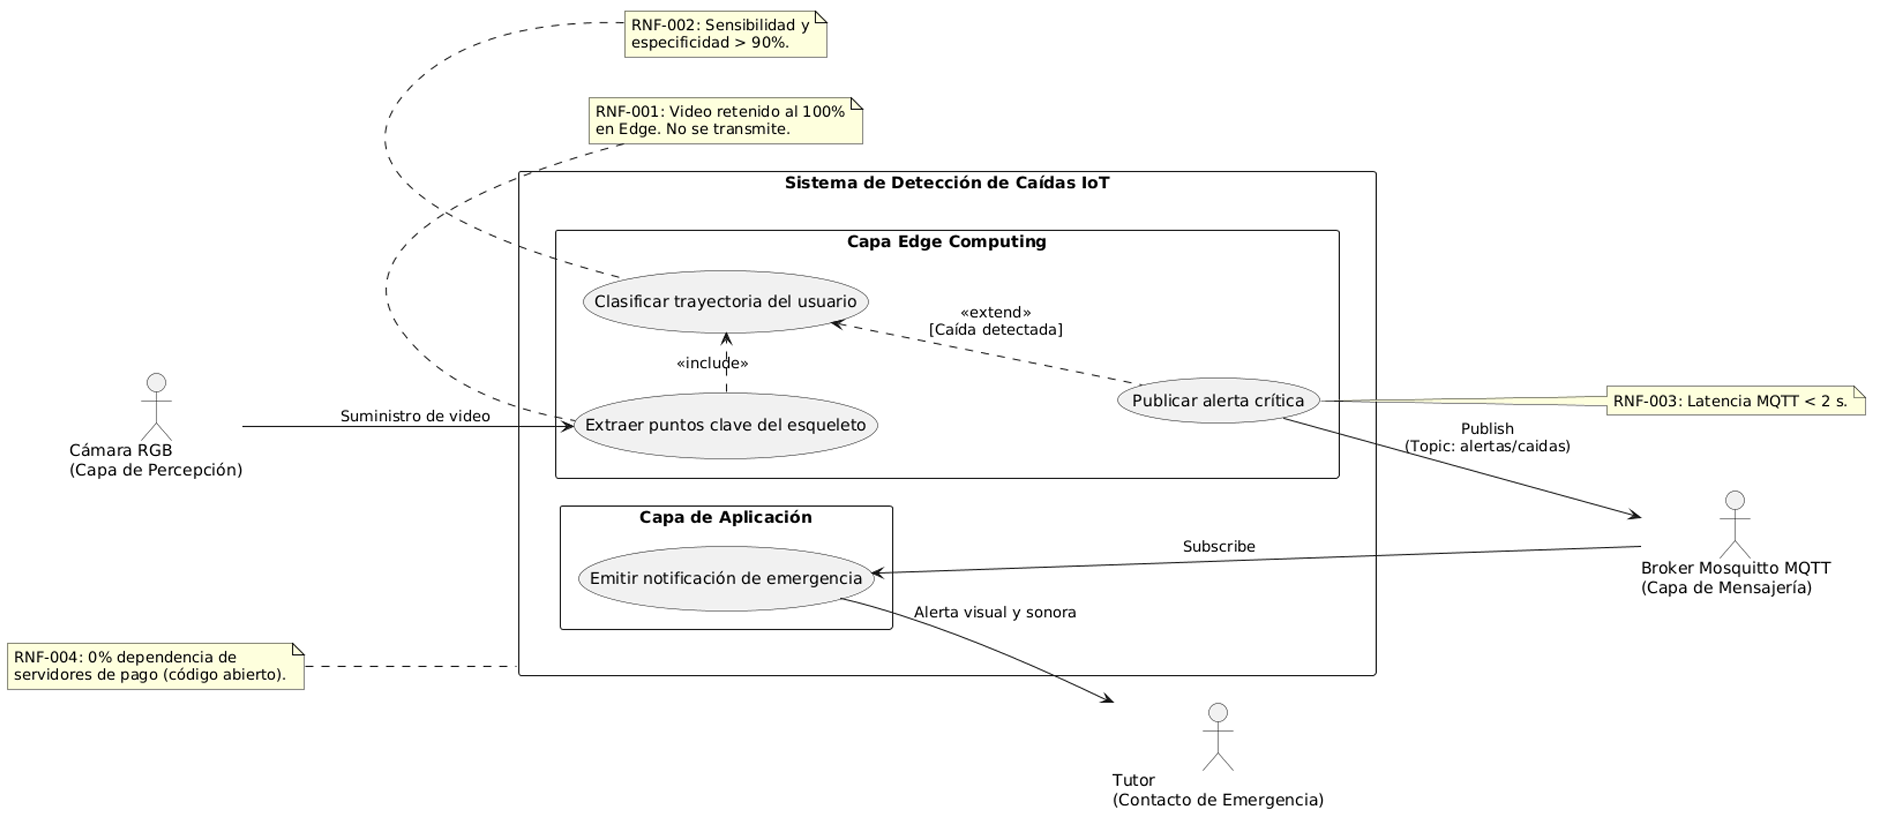
\includegraphics[width=\textwidth]{Figuras/casos_de_uso.png}
    \caption{Diagrama de casos de uso del sistema IoT.}
    \label{fig:casos_uso}
\end{sidewaysfigure}
\newpage


% ---------- Parte de María Fernanda (IA) ----------
\section{Requisitos del modelo de inteligencia artificial}
\label{sec:req-ia}

En esta sección se especifican los requisitos que debe cumplir el módulo de inteligencia artificial, es decir, el componente que recibe los cuadros de la cámara y decide si ocurrió una caída. Corresponden a la fase 1 de CRISP-ML(Q) (comprensión del negocio y de los datos) y sirven como referencia para evaluar el modelo en la fase 4.

\subsection{Requisitos funcionales}

\begin{table}[H]
\centering
\caption{Requisitos funcionales del modelo de IA.}
\label{tab:rf-ia}
\small
\begin{tabular}{L{1.9cm}L{6.6cm}L{1.8cm}}
\toprule
\textbf{ID} & \textbf{Descripción} & \textbf{Prioridad} \\
\midrule
RF-IA-01 & El módulo debe recibir cuadros RGB de una sola cámara en el formato acordado en el flujo de adquisición. & Alta \\
\addlinespace
RF-IA-02 & El módulo debe detectar a la persona presente en cada cuadro y estimar sus 17 puntos clave en formato COCO, con coordenadas $(x, y)$ y confianza. & Alta \\
\addlinespace
RF-IA-03 & El módulo debe clasificar la postura de la persona en cada cuadro como \textit{de pie}, \textit{sentado}, \textit{acostado} o \textit{caído}. & Alta \\
\addlinespace
RF-IA-04 & El módulo debe analizar la secuencia de posturas de los últimos segundos y determinar si corresponde a una \textit{caída} o a \textit{no caída}, con un nivel de confianza asociado. & Alta \\
\addlinespace
RF-IA-05 & El módulo debe distinguir una caída de actividades cotidianas similares: sentarse, acostarse, agacharse y recoger un objeto. & Alta \\
\addlinespace
RF-IA-06 & Al detectar una caída, el módulo debe entregar el evento (marca de tiempo y probabilidad) al componente de alertas en el formato acordado con el subsistema IoT. & Alta \\
\addlinespace
RF-IA-07 & El módulo debe descartar los cuadros en los que la confianza promedio de los puntos clave sea menor a un umbral, para no clasificar esqueletos incompletos. & Media \\
\bottomrule
\end{tabular}
\end{table}

\subsection{Requisitos no funcionales}

\begin{table}[H]
\centering
\caption{Requisitos no funcionales del modelo de IA.}
\label{tab:rnf-ia}
\small
\begin{tabular}{L{2.1cm}L{2.2cm}L{6.1cm}}
\toprule
\textbf{ID} & \textbf{Atributo} & \textbf{Descripción} \\
\midrule
RNF-IA-01 & Desempeño & El procesamiento completo (estimación de pose + clasificación) debe ejecutarse en la placa Edge a una tasa no menor a la fijada en los criterios de éxito (Tabla~\ref{tab:criterios-exito}). \\
\addlinespace
RNF-IA-02 & Portabilidad & El modelo debe poder exportarse a un formato ligero compatible con la placa Edge (por ejemplo, ONNX o TFLite), con precisión reducida (FP16 o INT8) si el hardware lo requiere. \\
\addlinespace
RNF-IA-03 & Eficiencia & El modelo debe caber en la memoria disponible de la placa sin impedir la ejecución del cliente MQTT y del sistema operativo. \\
\addlinespace
RNF-IA-04 & Privacidad & El video debe procesarse localmente en la placa; ningún cuadro debe enviarse fuera del dispositivo. Solo se transmite el evento de caída. \\
\addlinespace
RNF-IA-05 & Robustez & El modelo debe mantener las métricas objetivo con variaciones de iluminación interior y con la persona vista de frente, de lado o de espaldas. \\
\addlinespace
RNF-IA-06 & Trazabilidad & Cada experimento de entrenamiento debe registrar datos utilizados, hiperparámetros y métricas obtenidas, para que los resultados sean reproducibles. \\
\bottomrule
\end{tabular}
\end{table}

\subsection{Restricciones}

\begin{itemize}
  \item Se utiliza una sola cámara RGB convencional; no se emplean sensores de profundidad ni dispositivos portables.
  \item El sistema está pensado para un adulto mayor en una habitación; escenas con varias personas quedan fuera del alcance.
  \item Por la dificultad ética de obtener caídas reales de adultos mayores, el entrenamiento se basa en conjuntos de datos públicos con caídas simuladas \parencite{igual2013challenges,alam2022review}; esta limitación se mitiga con un conjunto de validación capturado en condiciones reales.
  \item La capacidad de cómputo y la memoria están limitadas por la placa Edge seleccionada, la Raspberry Pi 5, por lo que se priorizan las variantes compactas de YOLO26-pose \parencite{sapkota2025yolo26}.
\end{itemize}

\section{Métricas objetivo y criterios de éxito}
\label{sec:criterios-exito}

Los criterios de éxito son los valores contra los que se decidirá, en la fase de evaluación, si el prototipo cumple su objetivo. Se definieron de forma conjunta para el sistema completo: las métricas del modelo las establece el módulo de IA y los tiempos de respuesta, la infraestructura IoT. La Tabla~\ref{tab:criterios-exito} los resume.

\begin{table}[htbp]
\centering
\caption{Criterios de éxito del prototipo.}
\label{tab:criterios-exito}
\small
\begin{tabular}{L{1.3cm}L{3.3cm}L{2.0cm}L{4.5cm}}
\toprule
\textbf{ID} & \textbf{Criterio} & \textbf{Valor objetivo} & \textbf{Justificación} \\
\midrule
CE-01 & Sensibilidad (Ec.~\ref{eq:sensibilidad}) & $\geq 90$\,\% & Cada falso negativo es una caída sin atender; es la métrica prioritaria. \\
\addlinespace
CE-02 & Especificidad (Ec.~\ref{eq:especificidad}) & $\geq 90$\,\% & Limita las falsas alarmas ante actividades cotidianas, que son mucho más frecuentes que las caídas. \\
\addlinespace
CE-03 & Precisión (Ec.~\ref{eq:precision}) & $\geq 85$\,\% & Asegura que la mayoría de las alertas que recibe el tutor correspondan a caídas reales. \\
\addlinespace
CE-04 & Exactitud (Ec.~\ref{eq:exactitud}) & $\geq 90$\,\% & Desempeño global; se reporta junto con las demás por el desbalance de clases. \\
\addlinespace
CE-05 & Tasa de procesamiento en la Raspberry Pi 5 & $\geq 5$ FPS & Permite registrar varios cuadros durante el descenso del cuerpo, que ocurre en un intervalo breve. \\
\addlinespace
CE-06 & Tiempo de extremo a extremo (caída $\rightarrow$ notificación en el teléfono) & $\leq 8$ s & Permite que el tutor reaccione de inmediato. \textit{Criterio definido con el subsistema IoT.} \\
\bottomrule
\end{tabular}
\end{table}

Los valores de CE-01 a CE-04 se fijaron por debajo de los reportados en condiciones de laboratorio por trabajos similares, que alcanzan o superan el 90\,\% de exactitud \parencite{kwolek2014human,mobasheri2022fall}, porque la literatura señala que el rendimiento disminuye al pasar de caídas simuladas a condiciones reales \parencite{igual2013challenges}. Entre sensibilidad y especificidad se prioriza la sensibilidad: si durante el ajuste del umbral de decisión no es posible alcanzar ambas, se preferirá aceptar algunas falsas alarmas antes que dejar caídas sin detectar.

% ============================================================
\chapter{Diseño del sistema}
\label{cap:diseno}

\section{Arquitectura IoT y flujos de alerta}
\label{sec:arquitectura-iot}

Para dar solución a los requerimientos de protección de datos personales, el sistema asume una estricta jerarquía de \textit{Edge Computing} dividida en cuatro estratos funcionales:

\begin{enumerate}
    \item \textbf{Capa de Percepción:} Integrada por un nodo sensor visual (cámara RGB) conectado de manera cableada al dispositivo local, asegurando un suministro de imágenes ininterrumpido y exento de latencias de transmisión sobre red de área local (LAN).
    \item \textbf{Capa de Cómputo Edge:} Compuesta por una Raspberry Pi 5 que actúa como placa Edge perimetral, donde reside el módulo de inferencia de YOLO26. Esta capa delimita la "zona cero" de privacidad: procesa cada tensor visual, extrae la pose y destruye de inmediato las imágenes crudas directamente en memoria, impidiendo que material visual privado abandone el dispositivo.
    \item \textbf{Capa de Mensajería:} Representada por el servidor ligero Mosquitto MQTT \parencite{mqtt2026estandar}. Esta capa aísla la carga pesada (la imagen) de la carga liviana (el metadato de alerta) y rutea los mensajes JSON hacia LAN de forma instantánea tras clasificar exitosamente un riesgo de caída.
    \item \textbf{Capa de Aplicación:} Compuesta por un terminal móvil inteligente dotado de la aplicación nativa en Android \parencite{uv2026desarrollo}, el cual consume remotamente (bajo redes de área amplia o LAN) el tópico MQTT, habilitando al usuario final en tiempo real.
\end{enumerate}
\begin{figure}[H]
\centering
\begin{tikzpicture}[
    font=\sffamily\small,
    % Estilos de los nodos
    percep/.style={rectangle, draw=black, thick, rounded corners=3pt, minimum width=3.6cm, minimum height=1.2cm, align=center, fill=blue!10},
    edgebox/.style={rectangle, draw=black, thick, rounded corners=3pt, minimum width=3.6cm, minimum height=1.2cm, align=center, fill=teal!10},
    broker/.style={ellipse, draw=black, thick, minimum width=4.8cm, minimum height=1.5cm, align=center, fill=gray!15},
    appbox/.style={rectangle, draw=black, thick, rounded corners=3pt, minimum width=3.6cm, minimum height=1.2cm, align=center, fill=orange!10},
    arrow/.style={-{Stealth[length=2.5mm]}, thick, draw=black!80}
]

% Nodos
\node[percep] (cam) {\textbf{Capa de Percepción}\\Cámara RGB};
\node[edgebox, right=3.5cm of cam] (edge) {\textbf{Capa Edge Computing}\\Raspberry Pi 5\\(Docker)\\Inferencia YOLO26};
\node[broker, below=1.8cm of edge] (broker) {\textbf{Capa de Mensajería}\\Broker Mosquitto MQTT};
\node[appbox, below=1.8cm of cam] (app) {\textbf{Capa de Aplicación}\\App Móvil Android};

% Límite de privacidad (Recuadro rojo punteado)
\node[draw=red, dashed, thick, inner sep=12pt, fit=(edge),
      label={[text=red, font=\bfseries\footnotesize, align=center]above:Límite de Privacidad\\(Procesamiento local, no se almacena video)}] (privacy) {};

% Flechas y etiquetas
\draw[arrow] (cam) -- node[above, font=\footnotesize, align=center] {Video en vivo\\(USB/CSI)} (edge);

% La flecha hacia abajo lleva texto a la derecha
\draw[arrow] (edge) -- node[right, font=\footnotesize, align=center] {Publish: JSON\\(Topic: alertas/caidas)} (broker);

% La flecha hacia la izquierda lleva texto arriba
\draw[arrow] (broker) -- node[above, font=\footnotesize, align=center] {Subscribe\\(Wi-Fi)} (app);

\end{tikzpicture}
\caption{Diagrama de la arquitectura IoT.}
\label{fig:arquitectura_iot}
\end{figure}

\subsection{Estructura de tópicos MQTT y formato de mensajes}
La comunicación entre la Raspberry Pi 5 y la aplicación móvil se gestiona a través del \textit{broker} de código abierto \textbf{Eclipse Mosquitto} operando con nivel de calidad de servicio \textbf{QoS 1} (\textit{at least once}), lo que garantiza la recepción del mensaje de emergencia sin exceder el límite de latencia de red de 2 segundos (\textbf{RNF-003}). Se define la siguiente estructura de tópicos:

\begin{itemize}
    \item \texttt{alertas/caidas/\{device\_id\}}: Tópico principal en el que la placa Edge publica el evento positivo de caída y al cual permanece suscrita la aplicación móvil del tutor.
    \item \texttt{dispositivos/\{device\_id\}/estado}: Tópico destinado a reportar la disponibilidad de conexión del nodo perimetral (por ejemplo, el dispositivo \texttt{EG-014} en estado \textit{Conectado}).
\end{itemize}

Cuando el módulo de inteligencia artificial confirma una caída conforme a la regla temporal ($\Delta t \leq 2\text{ s}$ y permanencia en el suelo $N \geq 2\text{ s}$), entrega la marca de tiempo y el nivel de confianza (\textbf{RF-IA-06}) para construir la carga útil (\textit{payload}) en formato JSON que se muestra en el Listado~\ref{lst:json_alerta}.
\newpage

\begin{lstlisting}[caption={Estructura del paquete JSON publicado por la Raspberry Pi 5 ante una caída detectada.}, label={lst:json_alerta}]
{
  "device_id": "EG-014",
  "event_type": "FALL_DETECTED",
  "timestamp": "2026-10-12T10:18:00Z",
  "confidence": 0.94,
  "posture_state": "caido",
  "inactivity_seconds": 2.0
}
\end{lstlisting}

\subsection{Modelado de los flujos de alerta}
El comportamiento operativo del sistema ante la evaluación continua de secuencias de posturas se modela en tres flujos de decisión (Figura~\ref{fig:flujos_alerta}):

\begin{enumerate}
    \item \textbf{Flujo sin caída (actividad de la vida diaria):} Si el clasificador de posturas y la regla temporal determinan que la secuencia corresponde a una actividad cotidiana (caminar, sentarse, acostarse voluntariamente o agacharse momentáneamente por menos de $N$ segundos), la placa Edge omite cualquier publicación en red (\textbf{RF-004}), descarta los datos intermedios y continúa con el ciclo de adquisición.
    \item \textbf{Flujo de caída detectada:} Si se detecta una transición de \textit{de pie} o \textit{sentado} a \textit{caído} en un tiempo $\Delta t \leq 2\text{ s}$ seguida de al menos $N = 2\text{ s}$ en postura \textit{caído}, el módulo de IA emite el evento (\textbf{RF-IA-06}). El cliente MQTT de la placa publica el objeto JSON en el \textit{broker} Mosquitto (\textbf{RF-003}), el cual lo entrega de inmediato a la aplicación móvil para activar la alarma visual y sonora (\textbf{RF-005}) dentro de un tiempo total de extremo a extremo $\leq 8\text{ s}$ (\textbf{CE-06}).
    \item \textbf{Flujo de confirmación o descarte del tutor:} Al desplegarse la pantalla de alerta crítica en la aplicación móvil, el tutor evalúa la situación del adulto mayor y selecciona una de dos rutas:
    \begin{itemize}
        \item \textit{Confirmación de emergencia:} El tutor presiona \texttt{LLAMAR AL 911} para solicitar asistencia médica inmediata y el incidente queda asentado como alerta confirmada en la bitácora.
        \item \textit{Descarte por falsa alarma:} Si el tutor verifica que el adulto mayor se encuentra bien, presiona \texttt{Falsa Alarma}, silenciando la notificación y registrando el evento descartado en el historial para su análisis en la Fase 6 de CRISP-ML(Q).
    \end{itemize}
\end{enumerate}

\begin{figure}[htbp]
\centering
\begin{tikzpicture}[
    node distance=0.6cm and 0.9cm,
    every node/.style={font=\scriptsize},
    process/.style={rectangle, draw=black!80, fill=blue!6, rounded corners=3pt, minimum width=3.2cm, minimum height=0.85cm, align=center, thick},
    decision/.style={diamond, aspect=2.1, draw=black!80, fill=yellow!15, inner sep=1.5pt, align=center, thick},
    alert/.style={rectangle, draw=red!80!black, fill=red!10, rounded corners=3pt, minimum width=3.2cm, minimum height=0.85cm, align=center, thick},
    okblock/.style={rectangle, draw=green!60!black, fill=green!10, rounded corners=3pt, minimum width=3.2cm, minimum height=0.85cm, align=center, thick},
    arrow/.style={-{Stealth[length=2.2mm]}, thick, draw=black!80}
]

\node[process] (seq) {\textbf{Secuencia de posturas}\\Clasificador + ventana temporal};
\node[decision, below=of seq] (dec1) {¿Transición $\leq \Delta t$\\y caído $\geq N\text{ s}$?};

\node[okblock, right=1.4cm of dec1] (nocai) {\textbf{Flujo sin caída (RF-004)}\\Se omite envío MQTT y\\continúa captura local};

\node[alert, below=0.7cm of dec1] (pub) {\textbf{Flujo de caída (RF-003)}\\Publica JSON en Mosquitto\\Notificación en aplicación móvil};

\node[decision, below=of pub] (dec2) {Validación\\del tutor};

\node[alert, below left=0.6cm and 0.4cm of dec2] (conf) {\textbf{Confirmación}\\Llamada al 911\\Registro de incidente};
\node[okblock, below right=0.6cm and 0.4cm of dec2] (desc) {\textbf{Descarte (Falsa Alarma)}\\Cierra alerta activa\\Registro en bitácora (Fase 6)};

\draw[arrow] (seq) -- (dec1);
\draw[arrow] (dec1) -- node[above] {No (ADL)} (nocai);
\draw[arrow] (nocai.north) |- (seq.east);
\draw[arrow] (dec1) -- node[left] {Sí} (pub);
\draw[arrow] (pub) -- (dec2);
\draw[arrow] (dec2.west) -| node[above left] {Emergencia} (conf.north);
\draw[arrow] (dec2.east) -| node[above right] {Está bien} (desc.north);

\end{tikzpicture}
\caption{Diagrama de los flujos de decisión del sistema: sin caída, caída detectada y confirmación o descarte del tutor.}
\label{fig:flujos_alerta}
\end{figure}


\section{Selección de la plataforma de cómputo en el borde}
\label{sec:seleccion-placa}

La arquitectura de la Figura~\ref{fig:arquitectura_iot} reserva una capa de cómputo en el borde para ejecutar la estimación de pose, el clasificador de posturas, la regla temporal y el cliente MQTT, pero no impone un hardware específico. Para el prototipo se compararon cinco placas de desarrollo de uso común en proyectos de visión artificial y se seleccionó la Raspberry Pi 5. La evaluación se guio por seis criterios derivados de los requisitos de las Secciones~\ref{sec:req-sistema} y~\ref{sec:req-ia}: (1) capacidad de cómputo suficiente para sostener una tasa de al menos 5~FPS (CE-05); (2) memoria de al menos 4~GB para el modelo, el sistema operativo y el cliente de mensajería (RNF-IA-03); (3) soporte de los formatos de exportación de YOLO26-pose y de OpenCV (RNF-IA-02); (4) interfaz de cámara CSI o USB y conectividad Ethernet o Wi-Fi para publicar en el \textit{broker} (RNF-003); (5) costo y consumo eléctrico compatibles con el presupuesto del prototipo; y (6) disponibilidad de suministro y documentación técnica durante el periodo del proyecto.

\begin{table}[htbp]
\centering
\caption{Comparación de placas de desarrollo candidatas para la capa de cómputo en el borde.}
\label{tab:comparativa-placas}
\small
\begin{tabular}{L{2.5cm}L{2.7cm}L{2.3cm}L{1.1cm}L{1.6cm}L{2.3cm}}
\toprule
\textbf{Placa} & \textbf{CPU / GPU} & \textbf{Acelerador de IA} & \textbf{RAM} & \textbf{Costo (USD)} & \textbf{Resultado} \\
\midrule
Raspberry Pi 5 (8~GB) & 4 Cortex-A76 a 2,4~GHz; GPU VideoCore VII & Ninguno; Hailo-8L opcional por PCIe & 8~GB & 110--140 & Seleccionada \\
\addlinespace
Raspberry Pi 4 (4~GB) & 4 Cortex-A53 a 1,8~GHz; GPU VideoCore VI & Ninguno & 4~GB & 70--90 & Descartada: menor desempeño \\
\addlinespace
Jetson Orin Nano Super & 6 Cortex-A78AE; GPU Ampere & GPU, hasta 67 TOPS & 8~GB & $\approx$ 400 & Descartada: costo y consumo \\
\addlinespace
Coral Dev Board & 4 Cortex-A53 a 1,5~GHz & Edge TPU, 4 TOPS & 1~GB & 120--150 & Descartada: memoria y suministro \\
\addlinespace
Orange Pi 5 (8~GB) & 4 Cortex-A76 y 4 Cortex-A55; GPU Mali-G610 & NPU, 6 TOPS & 8~GB & 85--110 & Descartada: soporte del NPU \\
\bottomrule
\end{tabular}
\end{table}

Los datos técnicos de la Tabla~\ref{tab:comparativa-placas} provienen de las hojas de datos y de los sitios oficiales de cada fabricante \parencite{raspberrypi2026pi5,raspberrypi2026pi4,nvidia2026jetson,coral2026devboard,orangepi2026pi5}. Los costos son estimaciones a partir de los precios de lista de cada fabricante y de los ajustes de precio anunciados durante 2026, por lo que se emplean solo como orden de magnitud \parencite{raspberrypi2026precios}.

\paragraph{Raspberry Pi 5.} Se adopta la variante con 8~GB de memoria, que integra un procesador Broadcom BCM2712 de cuatro núcleos Arm Cortex-A76 a 2,4~GHz, memoria LPDDR4X, una GPU VideoCore VII, un puerto PCIe 2.0, dos conectores MIPI para cámara y pantalla, Ethernet Gigabit, Wi-Fi de doble banda, Bluetooth 5.0 y 40 pines de propósito general \parencite{raspberrypi2026pi5}. La placa no incluye una unidad de procesamiento neuronal, de modo que la inferencia se ejecuta en la CPU; esto es viable porque YOLO26 se diseñó para dispositivos de borde y puede exportarse a ONNX, TensorRT, TFLite o OpenVINO con cuantización de 8 bits \parencite{sapkota2025yolo26}. Si en la fase 3 de CRISP-ML(Q) la tasa de procesamiento no alcanza el criterio CE-05, el mismo puerto PCIe permite añadir un acelerador Hailo-8L de 13 TOPS sin cambiar de plataforma \parencite{raspberrypi2026aihat}. La variante de 8~GB se prefiere sobre las de 2 y 4~GB para dejar margen al sistema operativo, al contenedor de Docker, a OpenCV y al cliente MQTT, en cumplimiento del requisito RNF-IA-03, y se alimenta con una fuente USB-C de 5~V y 5~A (25~W) que cubre el consumo de la cámara y de la interfaz de red.

\paragraph{Alternativas descartadas.} La Raspberry Pi 4 tiene un costo menor, pero su procesador Cortex-A53 de cuatro núcleos a 1,8~GHz es de una generación anterior, carece de PCIe y no ofrece una ruta de ampliación si el modelo no alcanza la tasa requerida \parencite{raspberrypi2026pi4}; la diferencia de precio no compensa el menor desempeño. La Jetson Orin Nano Super es la opción más potente del conjunto, con hasta 67 TOPS en su GPU Ampere y 8~GB de memoria LPDDR5 \parencite{nvidia2026jetson}, pero cuesta alrededor del triple, consume hasta 25~W y su capacidad excede lo que necesita un modelo compacto que solo debe procesar entre 5 y 7 cuadros por segundo. La Coral Dev Board integra una Edge TPU de 4 TOPS con bajo consumo, pero limita la placa a 1~GB de memoria y exige convertir el modelo por completo a TFLite con cuantización entera, además de que su suministro y soporte se han reducido \parencite{coral2026devboard}. Por último, la Orange Pi 5 ofrece un procesador RK3588S con una NPU de 6 TOPS y un precio menor, pero su acelerador requiere la cadena de herramientas RKNN y su documentación y comunidad son más reducidas, lo que añade riesgo técnico a un proyecto con calendario fijo \parencite{orangepi2026pi5}.

\paragraph{Decisión.} Por lo anterior, la Raspberry Pi 5 de 8~GB se adopta como placa Edge del prototipo. La decisión no altera la arquitectura definida en la Sección~\ref{sec:arquitectura-iot}: la placa conserva el papel de capa de cómputo local, mantiene el procesamiento y el descarte de las imágenes dentro de la vivienda (RNF-001) y actúa como cliente publicador del \textit{broker} Mosquitto. El cumplimiento de los criterios CE-05 y CE-06 se verificará con mediciones sobre este hardware en la fase 3 de CRISP-ML(Q) y, si no se alcanza, se recurrirá al acelerador mencionado antes de considerar un cambio de plataforma.

\section{Flujo de adquisición de video}
\label{sec:flujo-adquisicion}

El flujo de adquisición de video parametriza la captura óptica en la Raspberry Pi 5 para suministrar cuadros de forma continua al módulo de inteligencia artificial, evitando cuellos de botella en la memoria y el procesador. Los parámetros de operación se definieron en conjunto con los requisitos del extractor de pose (\textbf{RF-IA-01}) y la estrategia de preprocesamiento en operación (Sección~\ref{sec:preproc-operacion}):

\begin{itemize}
    \item \textbf{Interfaz de captura y resolución de entrada:} La cámara RGB se conecta localmente mediante interfaz cableada (USB 2.0 / CSI) a la Raspberry Pi 5. La captura nativa se configura a una resolución base de $640 \times 480$ píxeles (relación de aspecto 4:3) y se redimensiona en memoria mediante OpenCV para que el lado mayor sea de $640\text{ píxeles}$, coincidiendo con la dimensión de entrada del modelo \texttt{YOLO26-pose}.
    \item \textbf{Tasa de cuadros por segundo (FPS):} El flujo de adquisición se regula a una tasa de captura sostenida de $5$ a $7\text{ FPS}$, garantizando una frecuencia de procesamiento en la placa superior al umbral mínimo establecido en los criterios de éxito (\textbf{CE-05}: $\geq 5\text{ FPS}$). Esta frecuencia temporal permite capturar con suficiente granularidad el descenso rápido del cuerpo durante una caída (intervalo $\Delta t \leq 2\text{ s}$) sin saturar la cola de lectura.
    \item \textbf{Formato de los cuadros en memoria (acuerdo con el módulo de IA):} La biblioteca OpenCV decodifica cada cuadro de la cámara como un arreglo matricial tridimensional de 8 bits por canal ($\texttt{uint8}$, con valores de intensidad entre $0$ y $255$) en orden de canales \texttt{BGR}. Antes de entregarse al modelo de estimación de pose, el arreglo se transforma en memoria RAM al espacio de color \texttt{RGB} con dimensiones $H \times W \times 3$.
    \item \textbf{Gestión de memoria volátil y privacidad:} En cumplimiento con los requisitos \textbf{RNF-001} y \textbf{RNF-IA-04}, no se realiza escritura de archivos de imagen ni de video en almacenamiento secundario. Se utiliza un búfer de lectura de un solo cuadro (\textit{single-frame buffer}) para descartar cuadros rezagados y procesar únicamente el instante actual; una vez extraídos los 17 puntos clave del esqueleto, el tensor de imagen se sobrescribe de inmediato en la memoria RAM.
\end{itemize}

La Figura~\ref{fig:flujo_adquisicion} ilustra la tubería de datos desde el sensor óptico hasta el módulo de inferencia local.

\begin{figure}[htbp]
\centering
\begin{tikzpicture}[
    node distance=0.65cm and 0.8cm,
    every node/.style={font=\footnotesize},
    block/.style={rectangle, draw=black!80, fill=blue!6, rounded corners=3pt, minimum width=3.4cm, minimum height=1.1cm, align=center, thick},
    edgeblock/.style={rectangle, draw=teal!80!black, fill=teal!8, rounded corners=3pt, minimum width=3.6cm, minimum height=1.1cm, align=center, thick},
    aiblock/.style={rectangle, draw=purple!80!black, fill=purple!8, rounded corners=3pt, minimum width=3.6cm, minimum height=1.1cm, align=center, thick},
    memblock/.style={rectangle, draw=red!80!black, fill=red!8, dashed, rounded corners=3pt, minimum width=3.6cm, minimum height=0.9cm, align=center, thick},
    arrow/.style={-{Stealth[length=2.5mm]}, thick, draw=black!80}
]

% Nodos
\node[block] (cam) {\textbf{Cámara RGB}\\Sensor óptico local\\Captura: $640 \times 480\text{ px}$\\Tasa: $5\text{--}7\text{ FPS}$};

\node[edgeblock, right=of cam] (opencv) {\textbf{Adquisición en Placa Edge}\\Lectura con OpenCV (RAM)\\Búfer de 1 cuadro (\texttt{uint8})\\Matriz \texttt{BGR} ($H \times W \times 3$)};

\node[edgeblock, below=of opencv] (preproc) {\textbf{Acondicionamiento de Formato}\\Conversión \texttt{BGR} $\rightarrow$ \texttt{RGB}\\Redimensionado a $640\text{ px}$\\Entrega en memoria (\textbf{RF-IA-01})};

\node[aiblock, left=of preproc] (yolo) {\textbf{Modelo YOLO26-pose}\\Inferencia en el borde\\Salida: 17 keypoints $(x, y, c)$\\en formato COCO (\textbf{RF-IA-02})};

\node[memblock, below=of preproc] (destroy) {\textbf{Liberación Volátil (RNF-001)}\\Destrucción inmediata del cuadro\\en RAM (0\,\% almacenamiento)};

% Flechas
\draw[arrow] (cam) -- node[above, font=\scriptsize] {USB / CSI} (opencv);
\draw[arrow] (opencv) -- (preproc);
\draw[arrow] (preproc) -- node[above, font=\scriptsize] {Tensor RGB} (yolo);
\draw[arrow] (yolo.south) |- (destroy.west);

\end{tikzpicture}
\caption{Diagrama de flujo de datos en la etapa de adquisición: Cámara $\rightarrow$ Placa Edge $\rightarrow$ Modelo de IA.}
\label{fig:flujo_adquisicion}
\end{figure}


\section{Estrategia de preprocesamiento de datos}
\label{sec:preprocesamiento}
 
El módulo de inteligencia artificial funciona en dos etapas: un clasificador que reconoce la postura de la persona en cada cuadro y un análisis temporal que decide, a partir de la secuencia de posturas, si ocurrió una caída (Sección~\ref{sec:secuencias}). En esta sección se describen el conjunto de datos seleccionado y el preprocesamiento que se aplica tanto para entrenar el clasificador como durante la operación del sistema.
 
\subsection{Conjunto de datos}
 
Como base se utiliza el \textit{Fall Detection Dataset} publicado en Kaggle \parencite{kandagatla2022fall}, que contiene 485 imágenes RGB, divididas en 374 para entrenamiento y 111 para validación. Cada imagen incluye la caja delimitadora de la persona y su etiqueta, en una de tres clases: \textit{Fall Detected}, \textit{Walking} y \textit{Sitting}. Se eligió porque es de acceso público y sus etiquetas corresponden directamente a posturas del cuerpo, lo que permite usarlo como punto de partida para el clasificador.
 
Las etiquetas originales se asignan a las posturas que reconocerá el clasificador, como se muestra en la Tabla~\ref{tab:clases-postura}. Dado que el conjunto no incluye la postura \textit{acostado}, indispensable para distinguir una caída de una persona que se recuesta voluntariamente, y que su tamaño es reducido, el conjunto se completará con imágenes de esa clase y con ejemplos adicionales de las demás, obtenidos de otros conjuntos públicos o capturados por el equipo en condiciones controladas.
 
\begin{table}[htbp]
\centering
\caption{Correspondencia entre las clases del conjunto de datos y las posturas del clasificador.}
\label{tab:clases-postura}
\small
\begin{tabular}{L{3.2cm}L{2.6cm}L{6.4cm}}
\toprule
\textbf{Clase original} & \textbf{Postura} & \textbf{Descripción} \\
\midrule
\textit{Walking} & De pie & Persona erguida, quieta o caminando. \\
\addlinespace
\textit{Sitting} & Sentado & Persona sentada en una silla, sillón o en el borde de la cama. \\
\addlinespace
--- (a completar) & Acostado & Persona recostada voluntariamente sobre una cama o un sillón. \\
\addlinespace
\textit{Fall Detected} & Caído & Persona en el suelo después de una caída. \\
\bottomrule
\end{tabular}
\end{table}
 
\subsection{Preprocesamiento para el entrenamiento}
 
Cada imagen del conjunto de datos pasa por los siguientes pasos para convertirse en un ejemplo de entrenamiento:
 
\begin{enumerate}
  \item \textbf{Revisión de calidad.} Se descartan las imágenes en las que la persona no es visible, aparece cortada por el borde o hay más de una persona, y se eliminan imágenes duplicadas o casi idénticas.
  \item \textbf{Estimación de pose.} Se aplica YOLO26-pose \parencite{ultralytics2026yolo26} para obtener los 17 puntos clave del esqueleto en formato COCO, cada uno con sus coordenadas $(x, y)$ y su confianza.
  \item \textbf{Asociación con la etiqueta.} Si el modelo detecta más de una persona, se conserva el esqueleto cuya caja delimitadora coincide mejor con la caja anotada en el conjunto de datos, de modo que la etiqueta corresponda al esqueleto correcto.
  \item \textbf{Filtrado por confianza.} Se descartan los esqueletos cuya confianza promedio sea menor a un umbral y se marcan como faltantes los puntos individuales con confianza baja, conforme al requisito RF-IA-07.
  \item \textbf{Normalización.} Las coordenadas se trasladan para que el punto medio de las caderas quede en el origen y se dividen entre la longitud del torso (distancia entre el punto medio de los hombros y el de las caderas). Así, el esqueleto no depende de la posición de la persona en la imagen ni de su distancia a la cámara.
  \item \textbf{Vector de características.} A las 34 coordenadas normalizadas se agregan características geométricas que ayudan a distinguir las posturas: el ángulo del tronco respecto a la vertical, la relación entre el alto y el ancho del esqueleto y la altura de la cabeza respecto a la cadera.
  \item \textbf{División de los datos.} Se conserva la división original en entrenamiento y validación, y se reserva un conjunto de prueba independiente formado por las imágenes capturadas por el equipo, para evaluar el modelo con datos que no provienen de la misma fuente.
\end{enumerate}
 
El balanceo de clases y el aumento de datos se realizarán en la fase 2 de TT2, una vez completado el conjunto.
 
\subsection{Preprocesamiento durante la operación}
\label{sec:preproc-operacion}
 
Durante el funcionamiento del prototipo, cada cuadro de la cámara sigue el mismo tratamiento que los datos de entrenamiento, de modo que el clasificador reciba entradas con las mismas características con las que fue entrenado:
 
\begin{enumerate}
  \item La cámara entrega cuadros a la tasa definida en el flujo de adquisición, con un mínimo de 5 cuadros por segundo (criterio CE-05).
  \item Cada cuadro se convierte a RGB y se redimensiona al tamaño de entrada de YOLO26-pose (640 píxeles en el lado mayor).
  \item Se estiman los puntos clave, se filtran por confianza y se normalizan como en el entrenamiento.
  \item El clasificador asigna una postura al cuadro. Para evitar cambios bruscos por errores aislados, se toma la postura mayoritaria en una ventana corta de cuadros.
  \item La postura se agrega a un historial de los últimos segundos, sobre el cual se aplica la regla temporal.
\end{enumerate}
 
\paragraph{Regla temporal.} Se considera que ocurrió una caída cuando se cumplen dos condiciones: (1) la persona pasa de \textit{de pie} o \textit{sentado} a \textit{caído} en un intervalo menor a $\Delta t$, y (2) permanece en la postura \textit{caído} durante al menos $N$ segundos. La primera condición distingue una caída de una persona que se recuesta poco a poco, y la segunda evita alertas por movimientos momentáneos, como agacharse a recoger un objeto. Como valores iniciales se proponen $\Delta t = 2$~s y $N = 2$~s, compatibles con el tiempo máximo de notificación del criterio CE-06; ambos se ajustarán durante la fase de evaluación. Cuando se cumplen las dos condiciones, el módulo entrega el evento de caída al componente de alertas (RF-IA-06).
 
Ningún cuadro se almacena: cada imagen se descarta en cuanto se extraen sus puntos clave, en congruencia con el requisito de privacidad RNF-IA-04.

\section{Diseño del extractor de pose}
\textit{[Pendiente: diseño del algoritmo de estimación de pose (María Fernanda, noviembre)]}

\section{Diseño de interfaces de la aplicación móvil Android}
\label{sec:mockups-app}

Con el propósito de cerrar el ciclo de notificación hacia el tutor, se diseñaron las interfaces de usuario (\textit{mockups}) de la aplicación móvil nativa para Android. El diseño prioriza una experiencia de usuario clara y de baja carga cognitiva, permitiendo gestionar el dispositivo de borde y reaccionar con rapidez ante una alerta de emergencia (\textbf{RF-005}).

\subsection{Registro del tutor y vinculación del dispositivo Edge}
El flujo inicial de configuración guía al tutor en tres pasos para dar de alta su cuenta y enlazar el nodo perimetral instalado en la vivienda del adulto mayor (Figura~\ref{fig:mockups_onboarding}):

\begin{enumerate}
    \item \textbf{Creación de cuenta y aviso de privacidad (Figura~\ref{fig:mockup1}):} Solicita las credenciales del tutor (correo electrónico y contraseña) y presenta de forma explícita el principio de \textit{Privacidad Local} (\textbf{RNF-001}), informando que las imágenes se procesan y permanecen en el dispositivo de cuidado y que únicamente se envían alertas de caída al teléfono móvil.
    \item \textbf{Descubrimiento y vinculación de hardware (Figura~\ref{fig:mockup2}):} Escanea e identifica los nodos disponibles en el entorno cercano (por ejemplo, los dispositivos \texttt{EG-014} y \texttt{EG-027}) para asociar el identificador único de la placa Edge con la suscripción al tópico MQTT correspondiente.
    \item \textbf{Personalización del perfil de cuidado (Figura~\ref{fig:mockup3}):} Permite asignar un nombre identificable al adulto mayor (por ejemplo, \textit{Abuelo José}) y un icono representativo asociado al dispositivo vinculado (\texttt{EG-014}).
\end{enumerate}

\begin{figure}[htbp]
\centering
\begin{subfigure}[b]{0.31\textwidth}
    \centering
    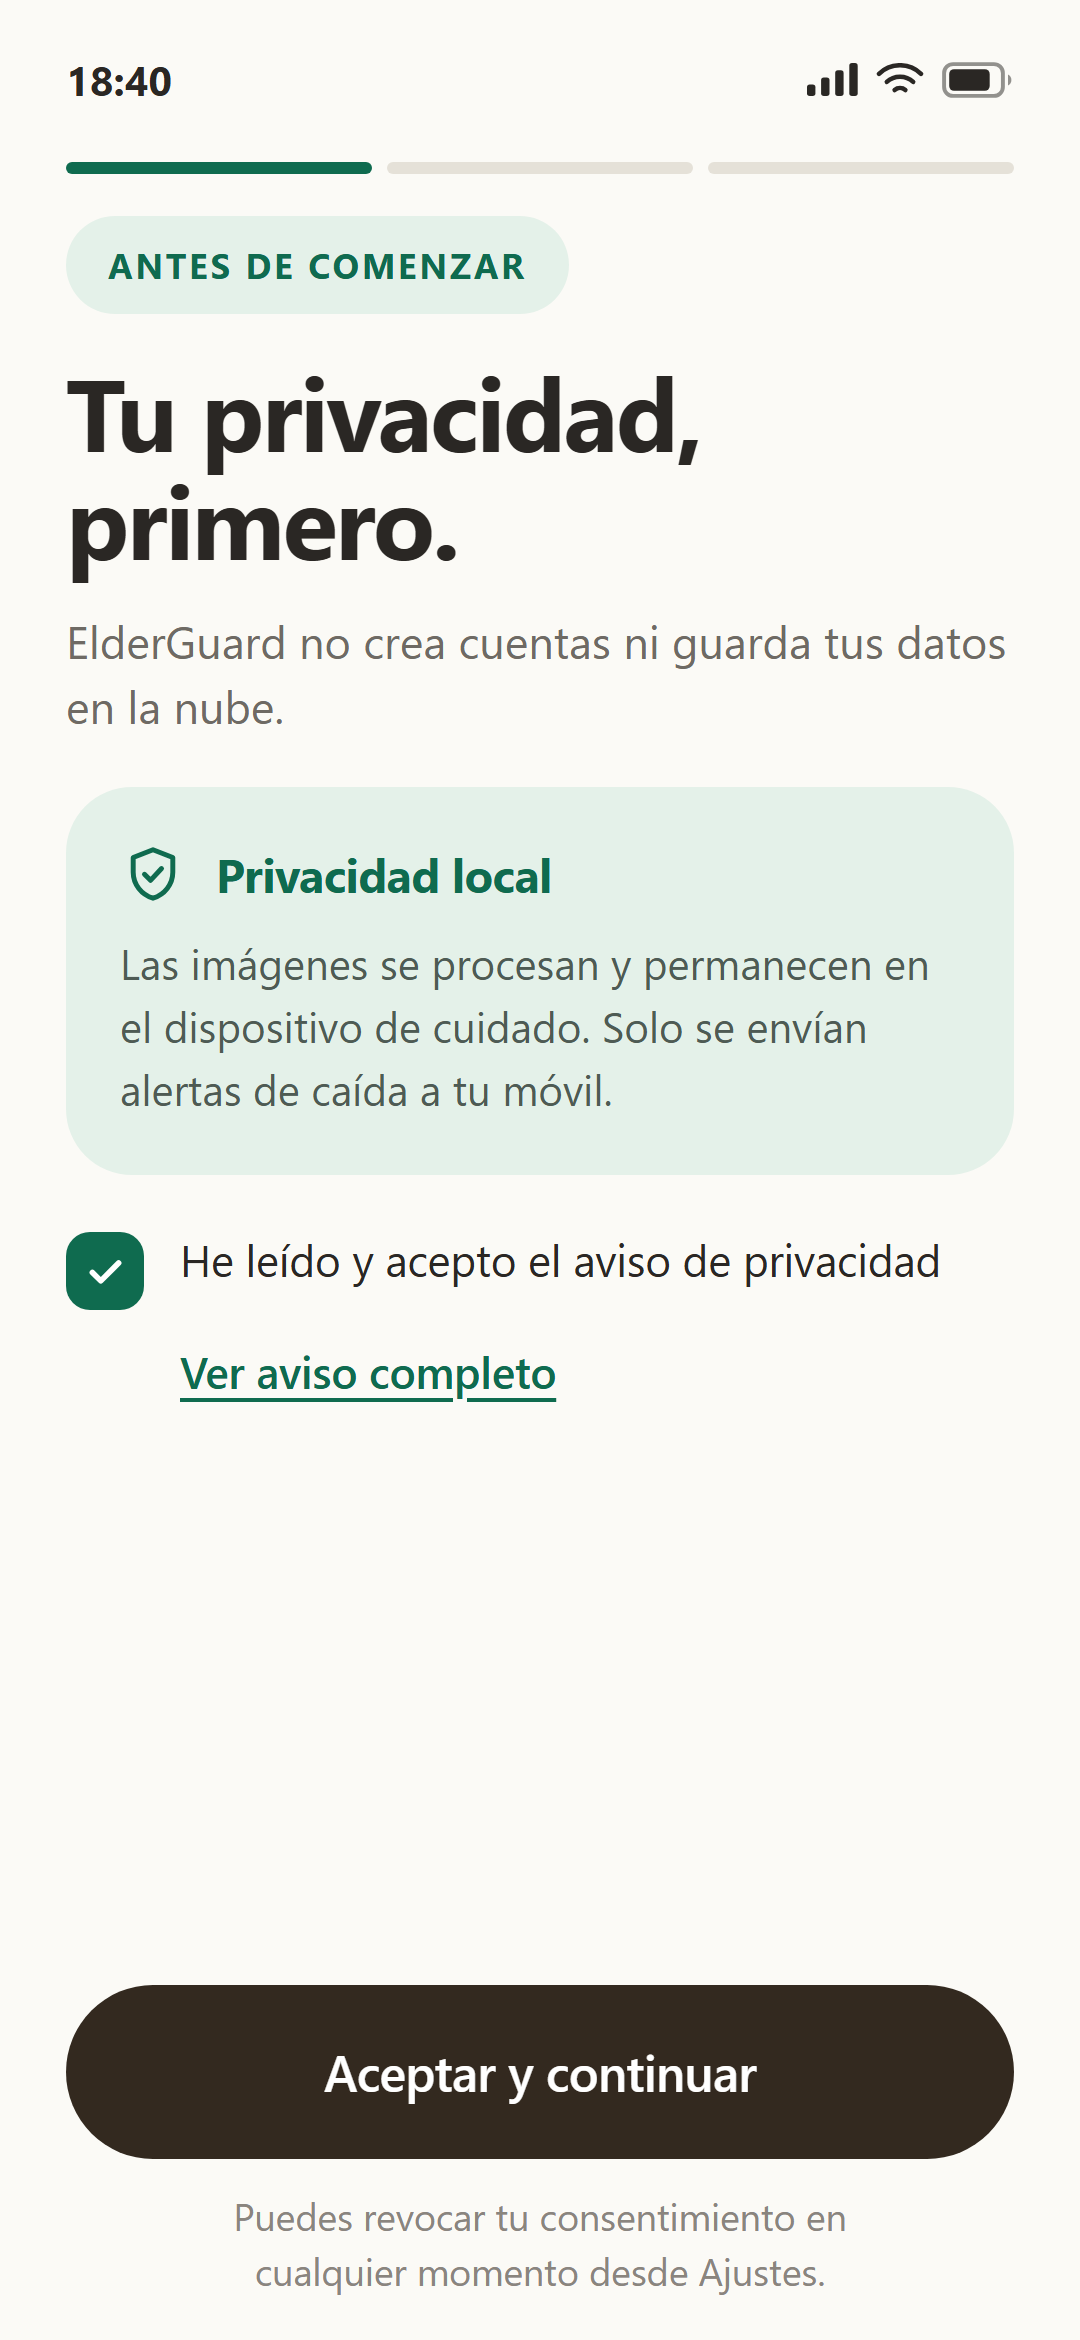
\includegraphics[width=\textwidth]{Figuras/mockup1.png}
    \caption{Registro de cuenta.}
    \label{fig:mockup1}
\end{subfigure}
\hfill
\begin{subfigure}[b]{0.31\textwidth}
    \centering
    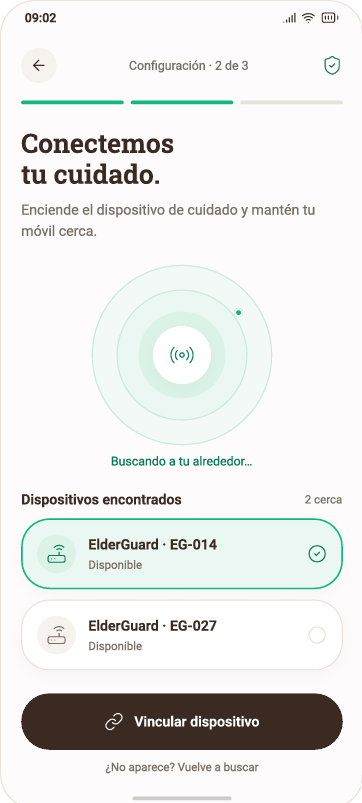
\includegraphics[width=\textwidth]{Figuras/mockup_2.png}
    \caption{Escaneo de nodos Edge.}
    \label{fig:mockup2}
\end{subfigure}
\hfill
\begin{subfigure}[b]{0.31\textwidth}
    \centering
    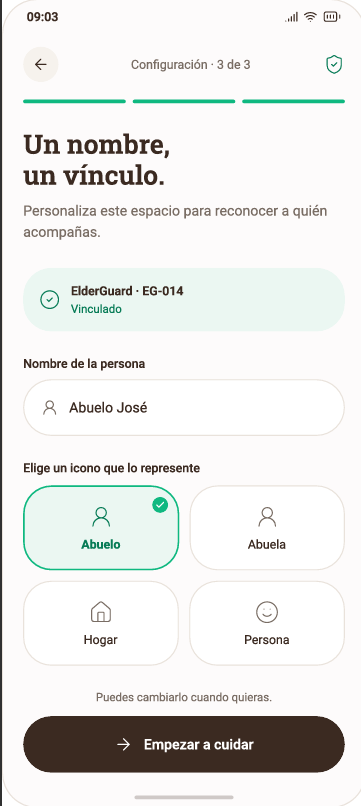
\includegraphics[width=\textwidth]{Figuras/mockup_3.png}
    \caption{Asignación de perfil.}
    \label{fig:mockup3}
\end{subfigure}
\caption{Mockups del flujo de registro y vinculación del dispositivo en la aplicación móvil.}
\label{fig:mockups_onboarding}
\end{figure}

\subsection{Monitoreo del estado, notificación crítica y bitácora de eventos}
Una vez configurado el dispositivo, la operación cotidiana y la atención de incidentes se estructuran en tres vistas principales de la aplicación móvil (Figura~\ref{fig:mockups_operacion}):

\begin{enumerate}
    \item \textbf{Panel principal de dispositivos conectados (Figura~\ref{fig:mockup4}):} Muestra el estado de enlace en tiempo real del nodo \texttt{EG-014} (\textit{Conectado}) asociado a \textit{Abuelo José}, reiterando la ausencia de transmisión de video y dando acceso directo a la adición de nuevos dispositivos y a la consulta del historial.
    \item \textbf{Pantalla de notificación crítica y validación/descarte (Figura~\ref{fig:mockup5}):} Al recibir un mensaje JSON de caída desde el \textit{broker} Mosquitto (\textbf{RF-003}, \textbf{RF-005}), la aplicación móvil despliega una alerta visual y sonora de alto contraste indicando \textit{``Posible caída detectada''}, el perfil afectado, el identificador del nodo (\texttt{EG-014}) y la hora del evento. La interfaz presenta dos acciones excluyentes para la validación humana:
    \begin{itemize}
        \item \textbf{Confirmar emergencia (\texttt{LLAMAR AL 911}):} Botón principal de alto contraste que inicia la llamada a los servicios de emergencia cuando el tutor confirma el accidente o no logra comunicarse con el adulto mayor.
        \item \textbf{Descartar evento (\texttt{Falsa Alarma}):} Acción secundaria que permite cerrar la alerta únicamente después de que el tutor verificó que el adulto mayor se encuentra bien.
    \end{itemize}
    \item \textbf{Historial y estado de los eventos (Figura~\ref{fig:mockup6}):} Registra cronológicamente la bitácora de actividad en la aplicación móvil mediante filtros por categoría (\textit{Todos}, \textit{Alerta resuelta}, \textit{Informativo}). Documenta tanto los eventos de conexión como la resolución de las alertas (por ejemplo, \textit{``Ana confirmó que José está bien. Falsa alarma registrada a las 10:21''}), proporcionando los registros necesarios para el análisis de falsos positivos contemplado en la Fase 6 de la metodología CRISP-ML(Q).
\end{enumerate}

\begin{figure}[htbp]
\centering
\begin{subfigure}[b]{0.31\textwidth}
    \centering
    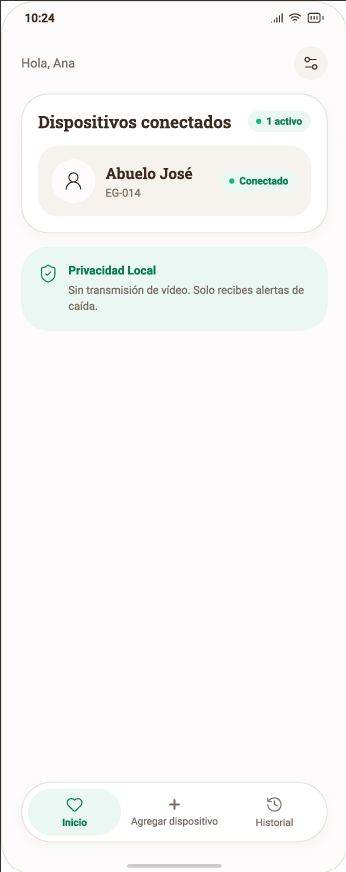
\includegraphics[width=\textwidth]{Figuras/mockup_4.png}
    \caption{Panel de estado activo.}
    \label{fig:mockup4}
\end{subfigure}
\hfill
\begin{subfigure}[b]{0.31\textwidth}
    \centering
    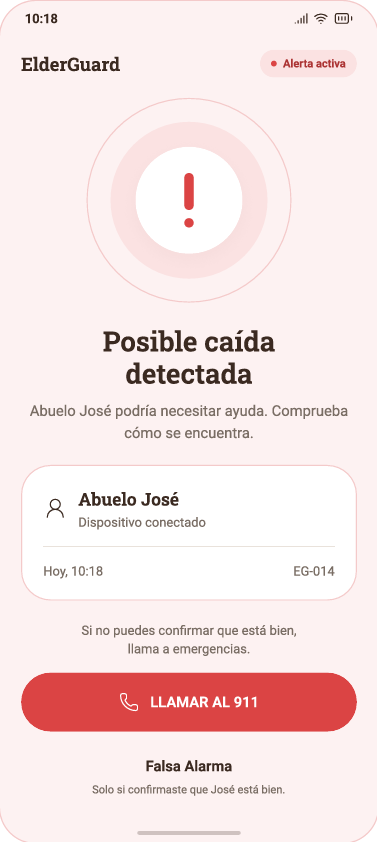
\includegraphics[width=\textwidth]{Figuras/mockup_5.png}
    \caption{Alerta crítica y validación.}
    \label{fig:mockup5}
\end{subfigure}
\hfill
\begin{subfigure}[b]{0.31\textwidth}
    \centering
    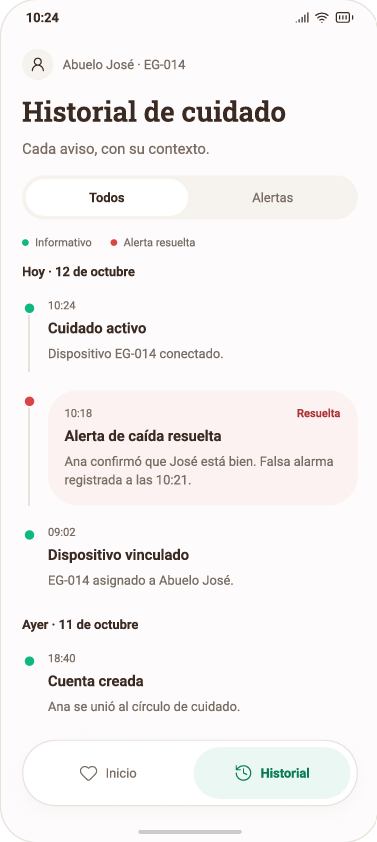
\includegraphics[width=\textwidth]{Figuras/mockup_6.png}
    \caption{Historial de eventos.}
    \label{fig:mockup6}
\end{subfigure}
\caption{Mockups de monitoreo, notificación crítica de caída y bitácora de eventos en la aplicación móvil.}
\label{fig:mockups_operacion}
\end{figure}

% ------------------------------------------------------------
%  BIBLIOGRAFÍA Y ANEXOS
% ------------------------------------------------------------
\backmatter
\printbibliography[heading=bibintoc,title={Referencias}]

\appendix
\chapter{Anexos}
\label{ap:material}

\end{document}